\chapter[]{I fazzoletti per istruzione militare in Italia}
\graphicspath{ {./images/chapter2/} }

\begin{figure}[h]
	\centering
		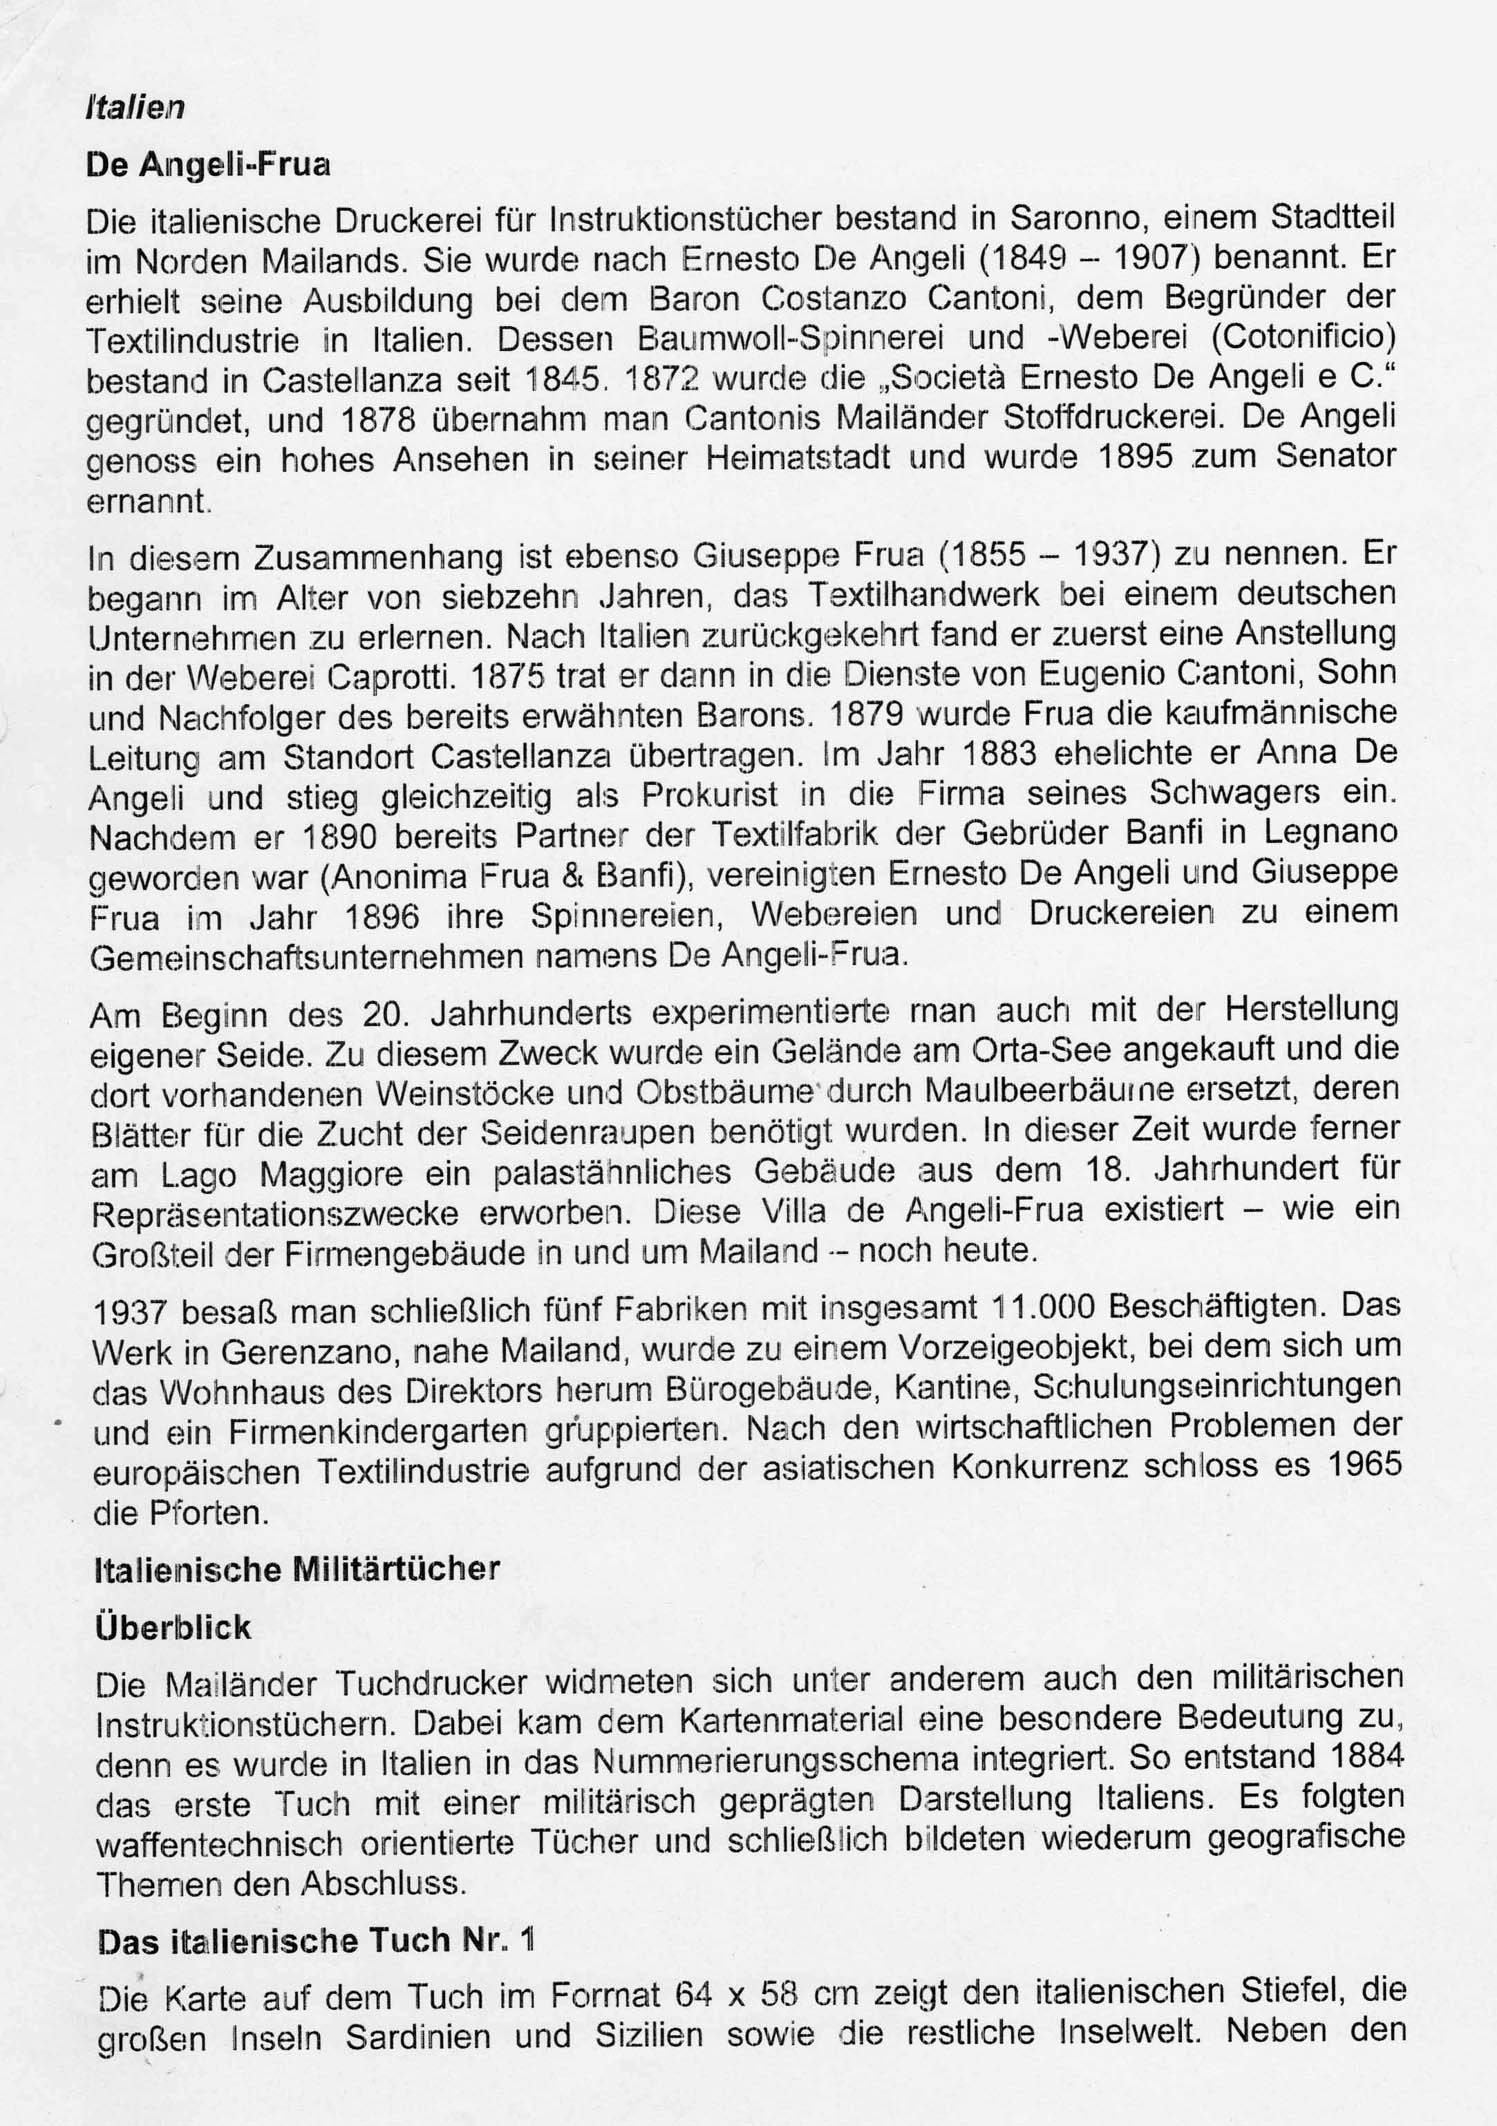
\includegraphics[width=\textwidth]{deangelifrua.jpg}
	\caption{}
	\label{fig:deangelifrua}
\end{figure}

\newpage

De Angeli-Frua

   La stamperia italiana per fazzoletti d'istruzione era a Saronno, una cittadina a nord di Milano. Era così chiamata dal nome di Ernesto De Angeli (1849-1907). Egli aveva ricevuto la sua formazione dal barone Costanzo Cantoni, il fondatore dell'industria tessile in Italia. La sua filanda e cotonificio era a Castellanza dal 1845. Nel 1872 fu fondata la "Società Ernesto De Angeli \& C." e nel 1878 si aprì la stamperia milanese di Cantoni. De Angeli raggiunse una grande reputazione e nel 1895 fu nominato Senatore.
   In questo contesto si deve citare anche Giuseppe Frua (1855-1937). Iniziò diciassettenne ad imparare la tessitura in un'impresa tedesca. Tornato in Italia trovò un primo impiego nel Cotonificio Caprotti. Nel 1875 entrò nella ditta di Eugenio Cantoni, figlio e successore del già menzionato barone. Nel 1879 Frua assunse la direzione commerciale della sede di Castellanza. Nel 1883 sposò Anna De Angeli e divenne Procuratore della ditta del cognato. Poi nel 1890 divenne socio della fabbrica tessile dei fratelli Banfi a Legnano (Anonima Frua \& Banfi), nel 1896 Ernesto De Angeli e Giuseppe Frua unirono le loro filature, cotonifici e stamperie in una società denominata De Angeli-Frua.
   All'inizio del XX secolo sperimentò anche la fabbricazione della seta. A questo fine fu acquistato un terreno sul lago d'Orta e furono sostituiti i vigneti ed i frutteti con piante di gelso, delle cui foglie vi era necessità per l'allevamento dei bachi da seta. Inoltre, in quel tempo fu acquistato sul Lago Maggiore un palazzetto del 18° secolo a scopo di rappresentanza. Questa villa De Angeli Frua esistette, come parte della ditta a Milano, fino ad oggi.
   Nel 1937 si contavano 5 fabbriche con 11000 addetti. Lo stabilimento di Gerenzano, vicino a Milano, fu un fiore all'occhiello, nel quale intorno all'abitazione del Direttore stavano edifici per uffici, mensa, scolastici ed un asilo aziendale. In seguito ai problemi economici dell'industria tessile europea nei confronti della concorrenza asiatica, chiuse nel 1965.


I fazzoletti militari Itaiani

Sguardo d'insieme
  
 Lo stampatore di fazzoletti milanese si dedicò anche ai fazzoletti d'istruzione militare. Il materiale cartografico è particolarmente importante, perché fu inserito in Italia in uno schema numerico. Così nel 1884 nacque in Italia il primo fazzoletto ad impronta militare. Seguirono fazzoletti indirizzati alla tecnica militare ed infine con temi geografici.

\newpage

Il fazzoletto italiano n°1 (vedi pag. 40)
  
 La mappa riprodotta sul fazzoletto nel formato 64 x 58 cm mostra lo stivale italiano, le grandi isole di Sardegna e Sicilia e il resto dell'arcipelago.
 
\begin{figure}[h]
	\centering
		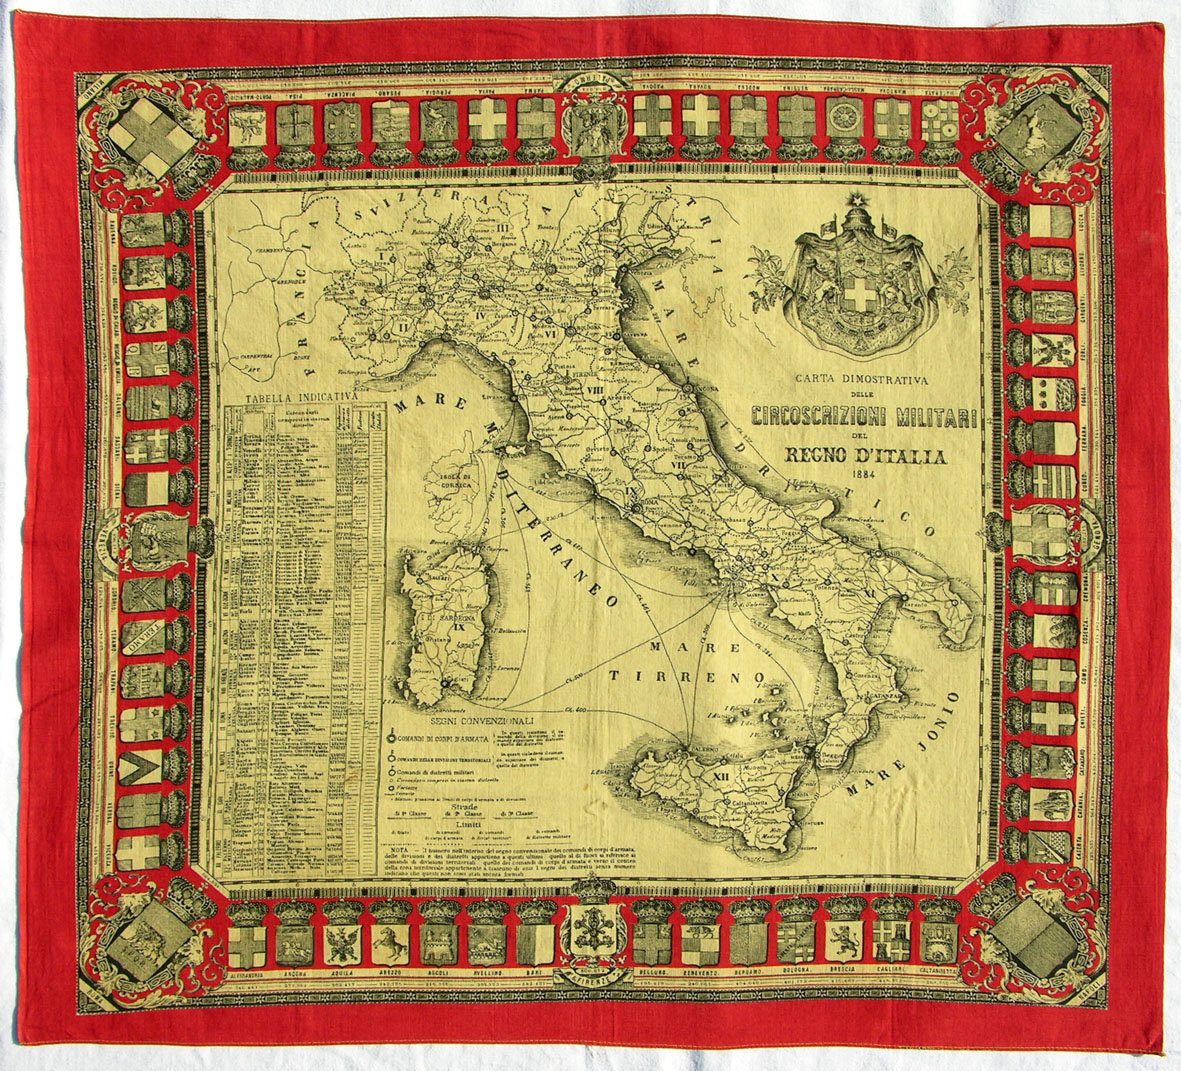
\includegraphics[width=\textwidth]{fazzoletto1_cartaitalia.jpg}
	\caption{Carta d’Italia 1884 Fazzoletto militare italiano n°1 Stamperia De Angeli – Milano}
	\label{fig:fazzoletto1_cartaitalia}
\end{figure}

\newpage

\begin{figure}[h]
	\centering
		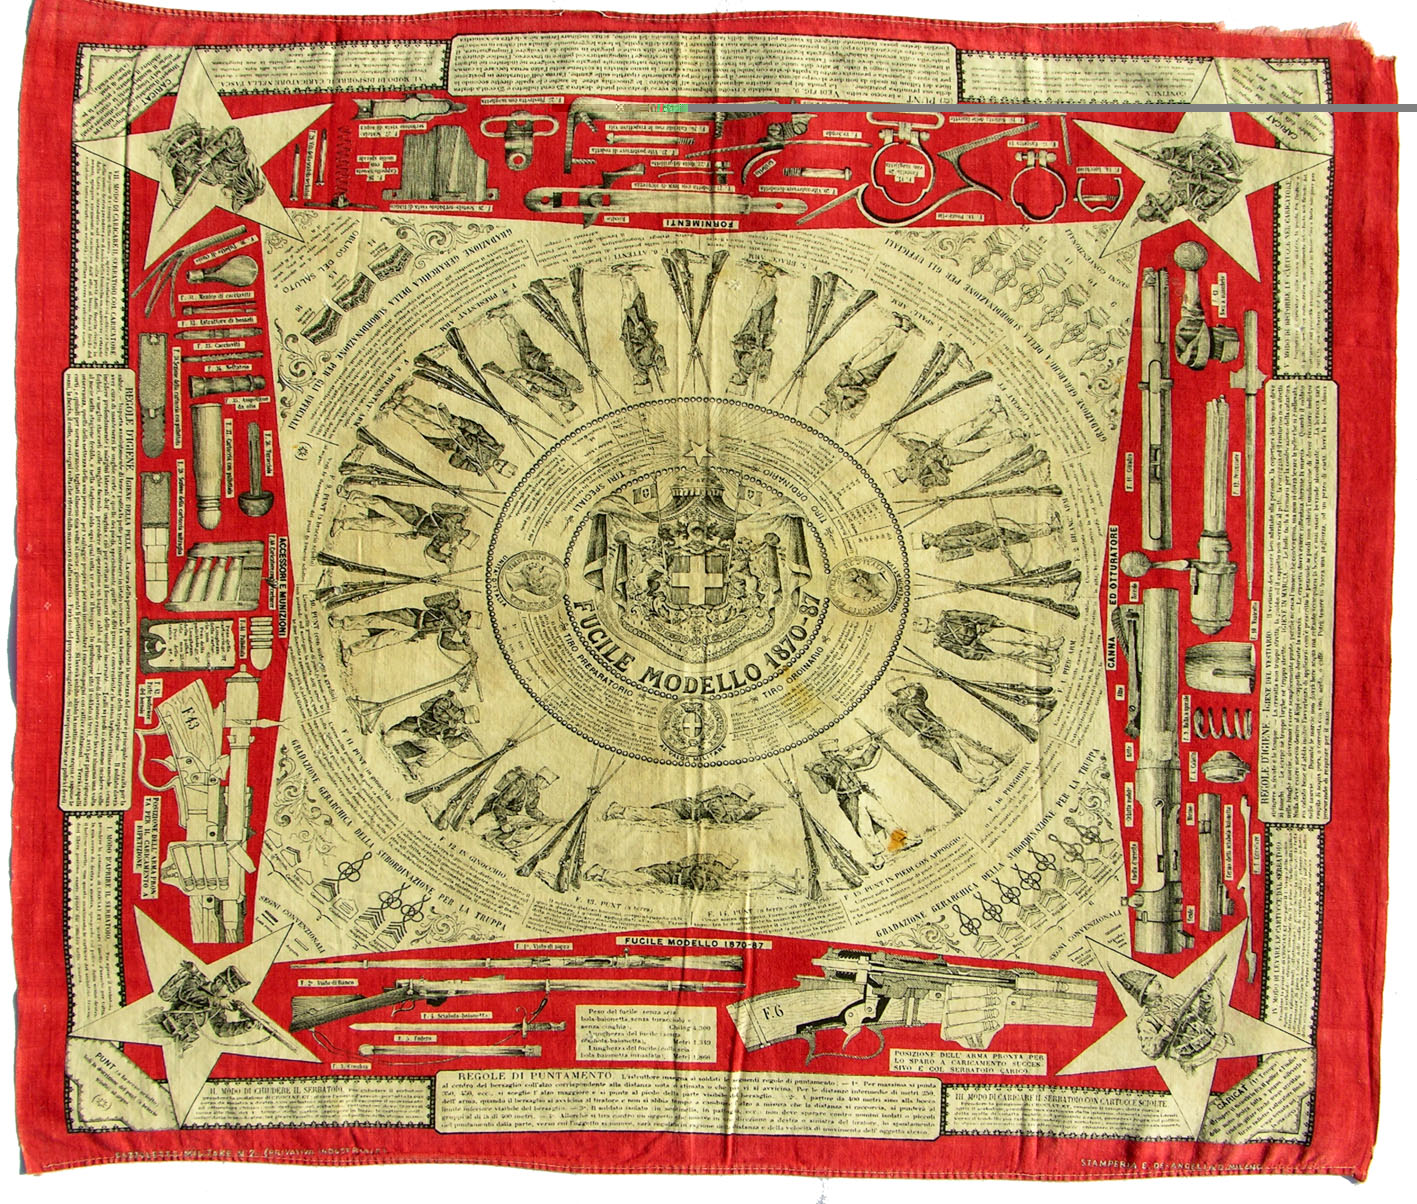
\includegraphics[width=\textwidth]{fazzoletto2.jpg}
	\caption{Fazzoletto militare italiano n°2 Stamperia De Angeli – Milano}
	\label{fig:fazzoletto2}
\end{figure}

\newpage

\begin{figure}[h]
	\centering
		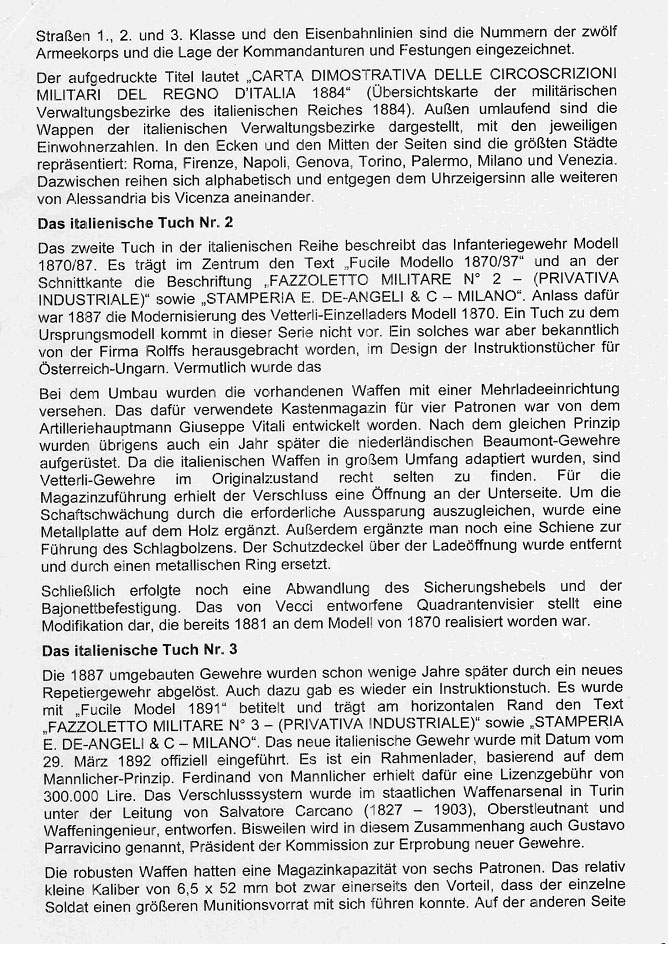
\includegraphics[width=\textwidth]{deangelifrua_2.jpg}
	\caption{}
	\label{fig:deangelifrua_2}
\end{figure}

\newpage

Oltre alle strade di 1a, 2a e 3a classe e le linee ferroviarie, compaiono i numeri dei dodici corpi d'armata dell'esercito e la posizione dei posti di comando e delle fortificazioni.
   II titolo stampato recita "CARTA DIMOSTRATIVA DELLE CIRCOSCRIZIONI MILITARI DEL REGNO D'ITALIA 1884" (mappa panoramica delle circoscrizioni militari del Regno d'Italia nel 1884). Sulla circonferenza esterna sono rappresentati gli stemmi dei distretti italiani, con i dati della popolazione. Negli angoli e al centro dei lati sono rappresentate le maggiori città: Roma, Firenze, Napoli, Genova, Torino, Palermo, Milano e Venezia. Esse sono allineate in ordine alfabetico e in senso antiorario da Alessandria a Vicenza.

Il fazzoletto italiano n°2 (vedi pag. 41)
  
 II secondo fazzoletto della serie italiana descrive il modello del fucile 1870/87 Nel centro figura il testo "Fucile Modello 1870/87" e sul bordo “FAZZOLETTO MILITARE N° 2 - (PRIVATIVA INDUSTRIALE)” e "STAMPERIA E. DE ANGELI \& C - MILANO". L'occasione fu quella, nel 1887, dell'ammodernamento del modello Vetterli del 1870. Un fazzoletto relativo a questo modello non è disponibile. Esso era stato prodotto dalla ditta Rolffs,(vedi pag. 44) come modello dei fazzoletti di istruzioni per l'Austria-Ungheria. 
   All'atto del miglioramento, le armi esistenti sono state dotate di un caricatore multiplo. Il caricatore utilizzato per quattro cartucce era stato sviluppato dal capitano d'artiglieria Giuseppe Vitali. Seguendo lo stesso principio un anno dopo, furono aggiornate le armi olandesi Beaumont. Dal momento che le armi italiane sono state adattate in larga misura, fucili Vetterli in condizioni originali sono abbastanza rari da trovare. II caricatore per l'alimentazione è dotato di un'apertura sul fondo. Per compensare l'indebolimento del fusto, una lastra di metallo è stata aggiunta al legno. Inoltre, si aggiunse una guida per il percussore. Il coperchio di protezione del carico superiore è stato rimosso e sostituito da un anello metallico. 
   Infine, c'è stata una variazione della sicura e della baionetta. Il mirino a quadrante elaborato da Vecci rappresenta una modifica che è stata attuata nel 1881 sul modello del 1870.

Il fazzoletto italiano N°3 (vedi pag. 45)
  
 I fucili 1887 sono stati sostituiti pochi anni dopo con un nuovo fucile a ripetizione. Inoltre, ci fu ancora una volta un fazzoletto di istruzioni. E' intitolato "Fucile Modello 1891” e porta sul bordo orizzontale il testo "FAZZOLETTO MILITARE n ° 3 - (PRIVATIVA INDUSTRIALE)" e “STAMPERIA E. DE ANGELI \& C – MILANO”. 
   Il nuovo fucile italiano è stato introdotto in data 29 Marzo 1892. Si tratta di un caricatore basato sul principio Mannlicher. Ferdinand von Mannlicher si era aggiudicata una fornitura di 300.000 lire. L'otturatore era stato progettato nell'arsenale di Torino da Salvatore Carcano (1827-1903), tenente colonnello e costruttore di armi. A volte viene richiamato in questo contesto, anche il nome di Gustavo Parravicino, Presidente della Commissione per la sperimentazione della nuova arma.
   
\newpage

La robusta arma aveva una capacità di sei pallottole. Il calibro relativamente piccolo di 6,5 x 52 mm, da un lato, ha offerto il vantaggio a ciascun soldato di poter portare con sé una maggiore quantità di munizioni.

\begin{figure}[h]
	\centering
		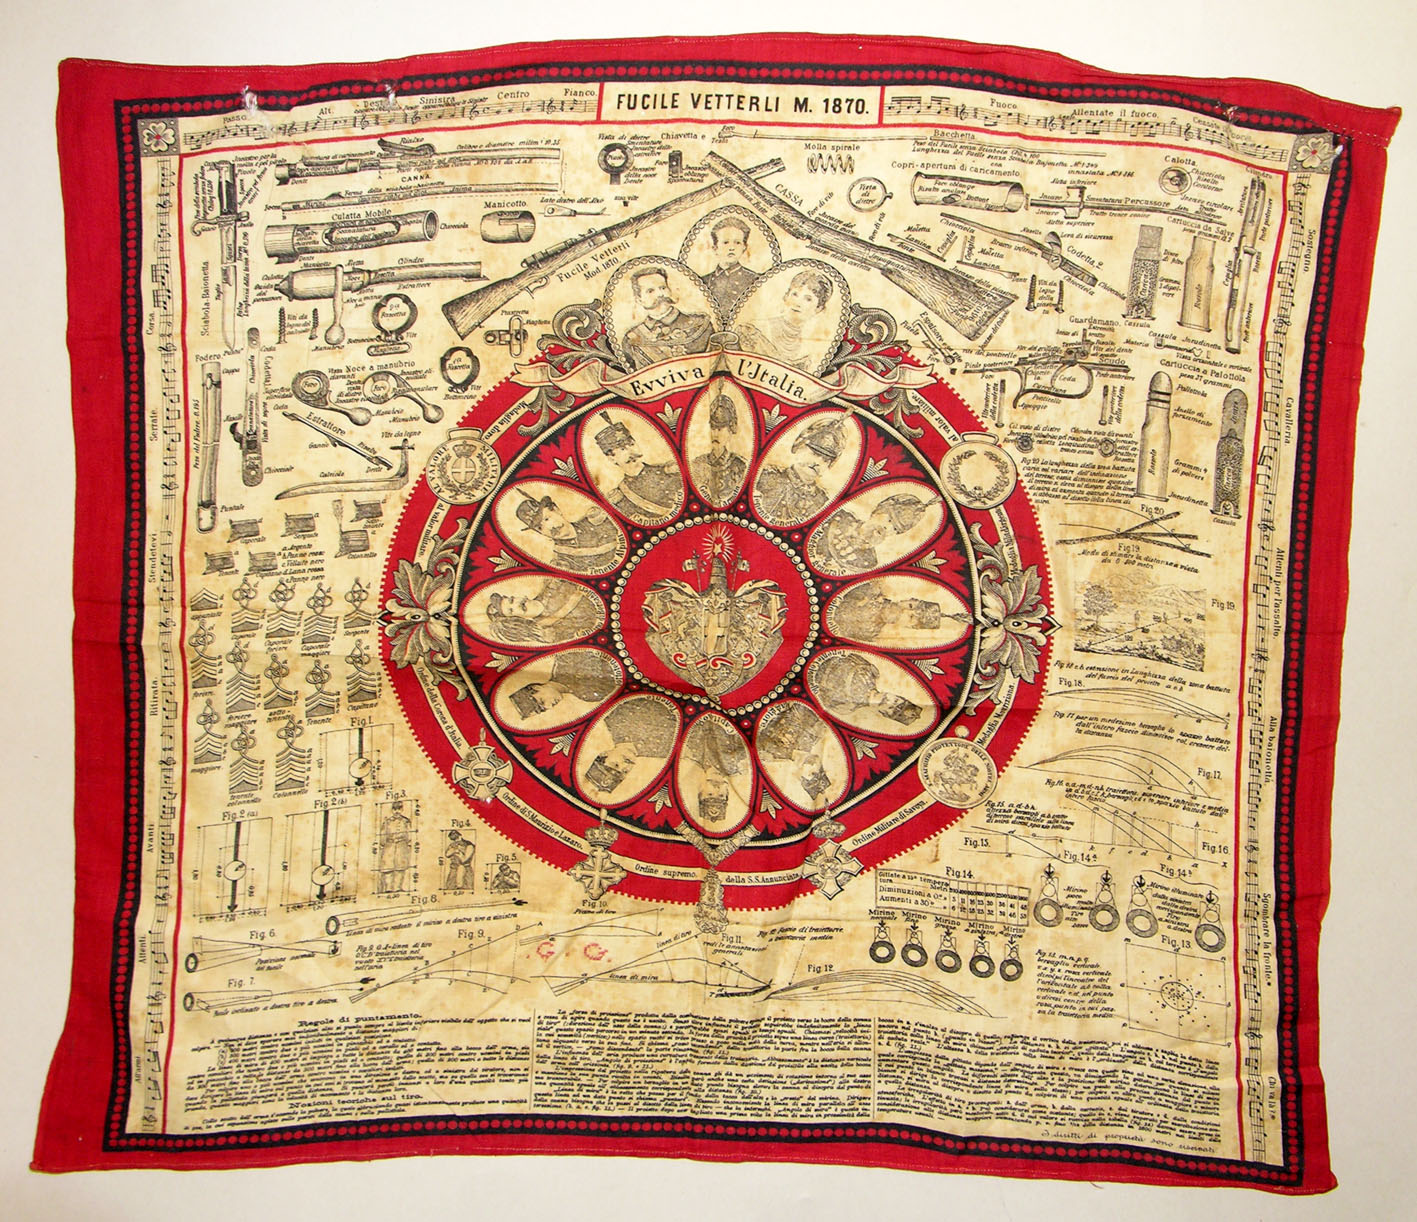
\includegraphics[width=\textwidth]{fazzoletto2A_rollfs.jpg}
	\caption{Fazzoletto militare n° 2A Rolffs \& Co.}
	\label{fig:fazzoletto2A_rollfs}
\end{figure}

\newpage

\begin{figure}[h]
	\centering
		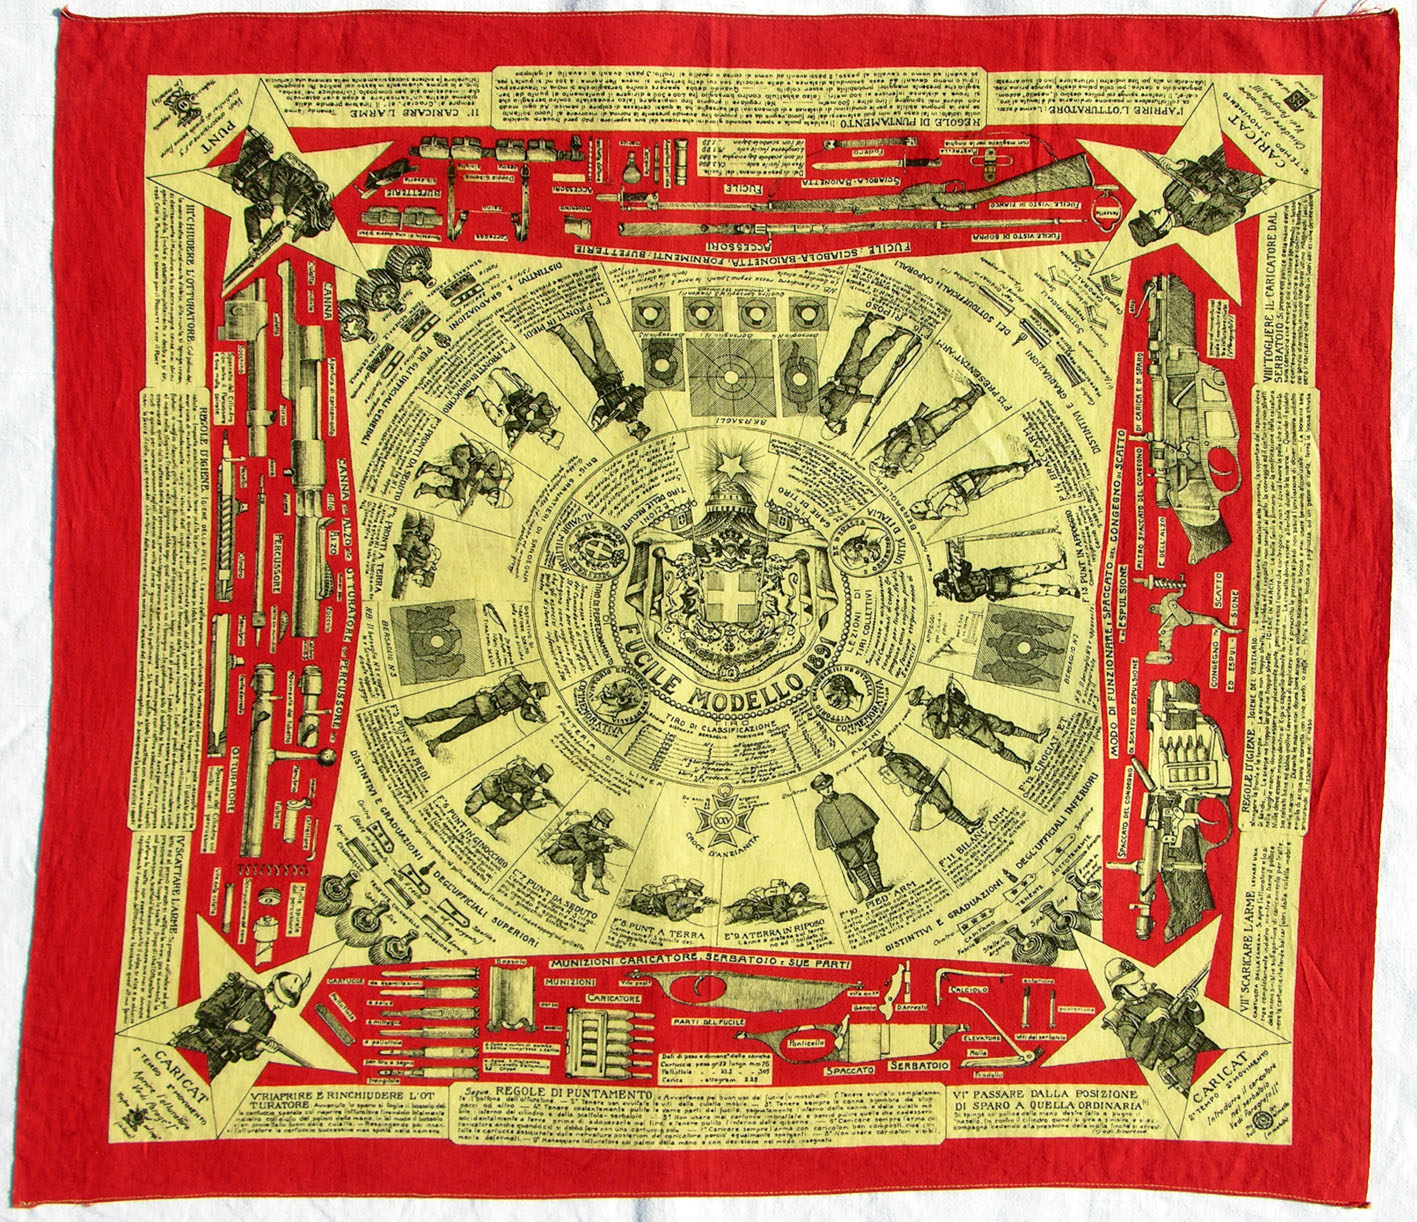
\includegraphics[width=\textwidth]{fazzoletto3.jpg}
	\caption{Fazzoletto militare italiano n°3. Stamperia De Angeli – Milano}
	\label{fig:fazzoletto3}
\end{figure}

\newpage

\begin{figure}[h]
	\centering
		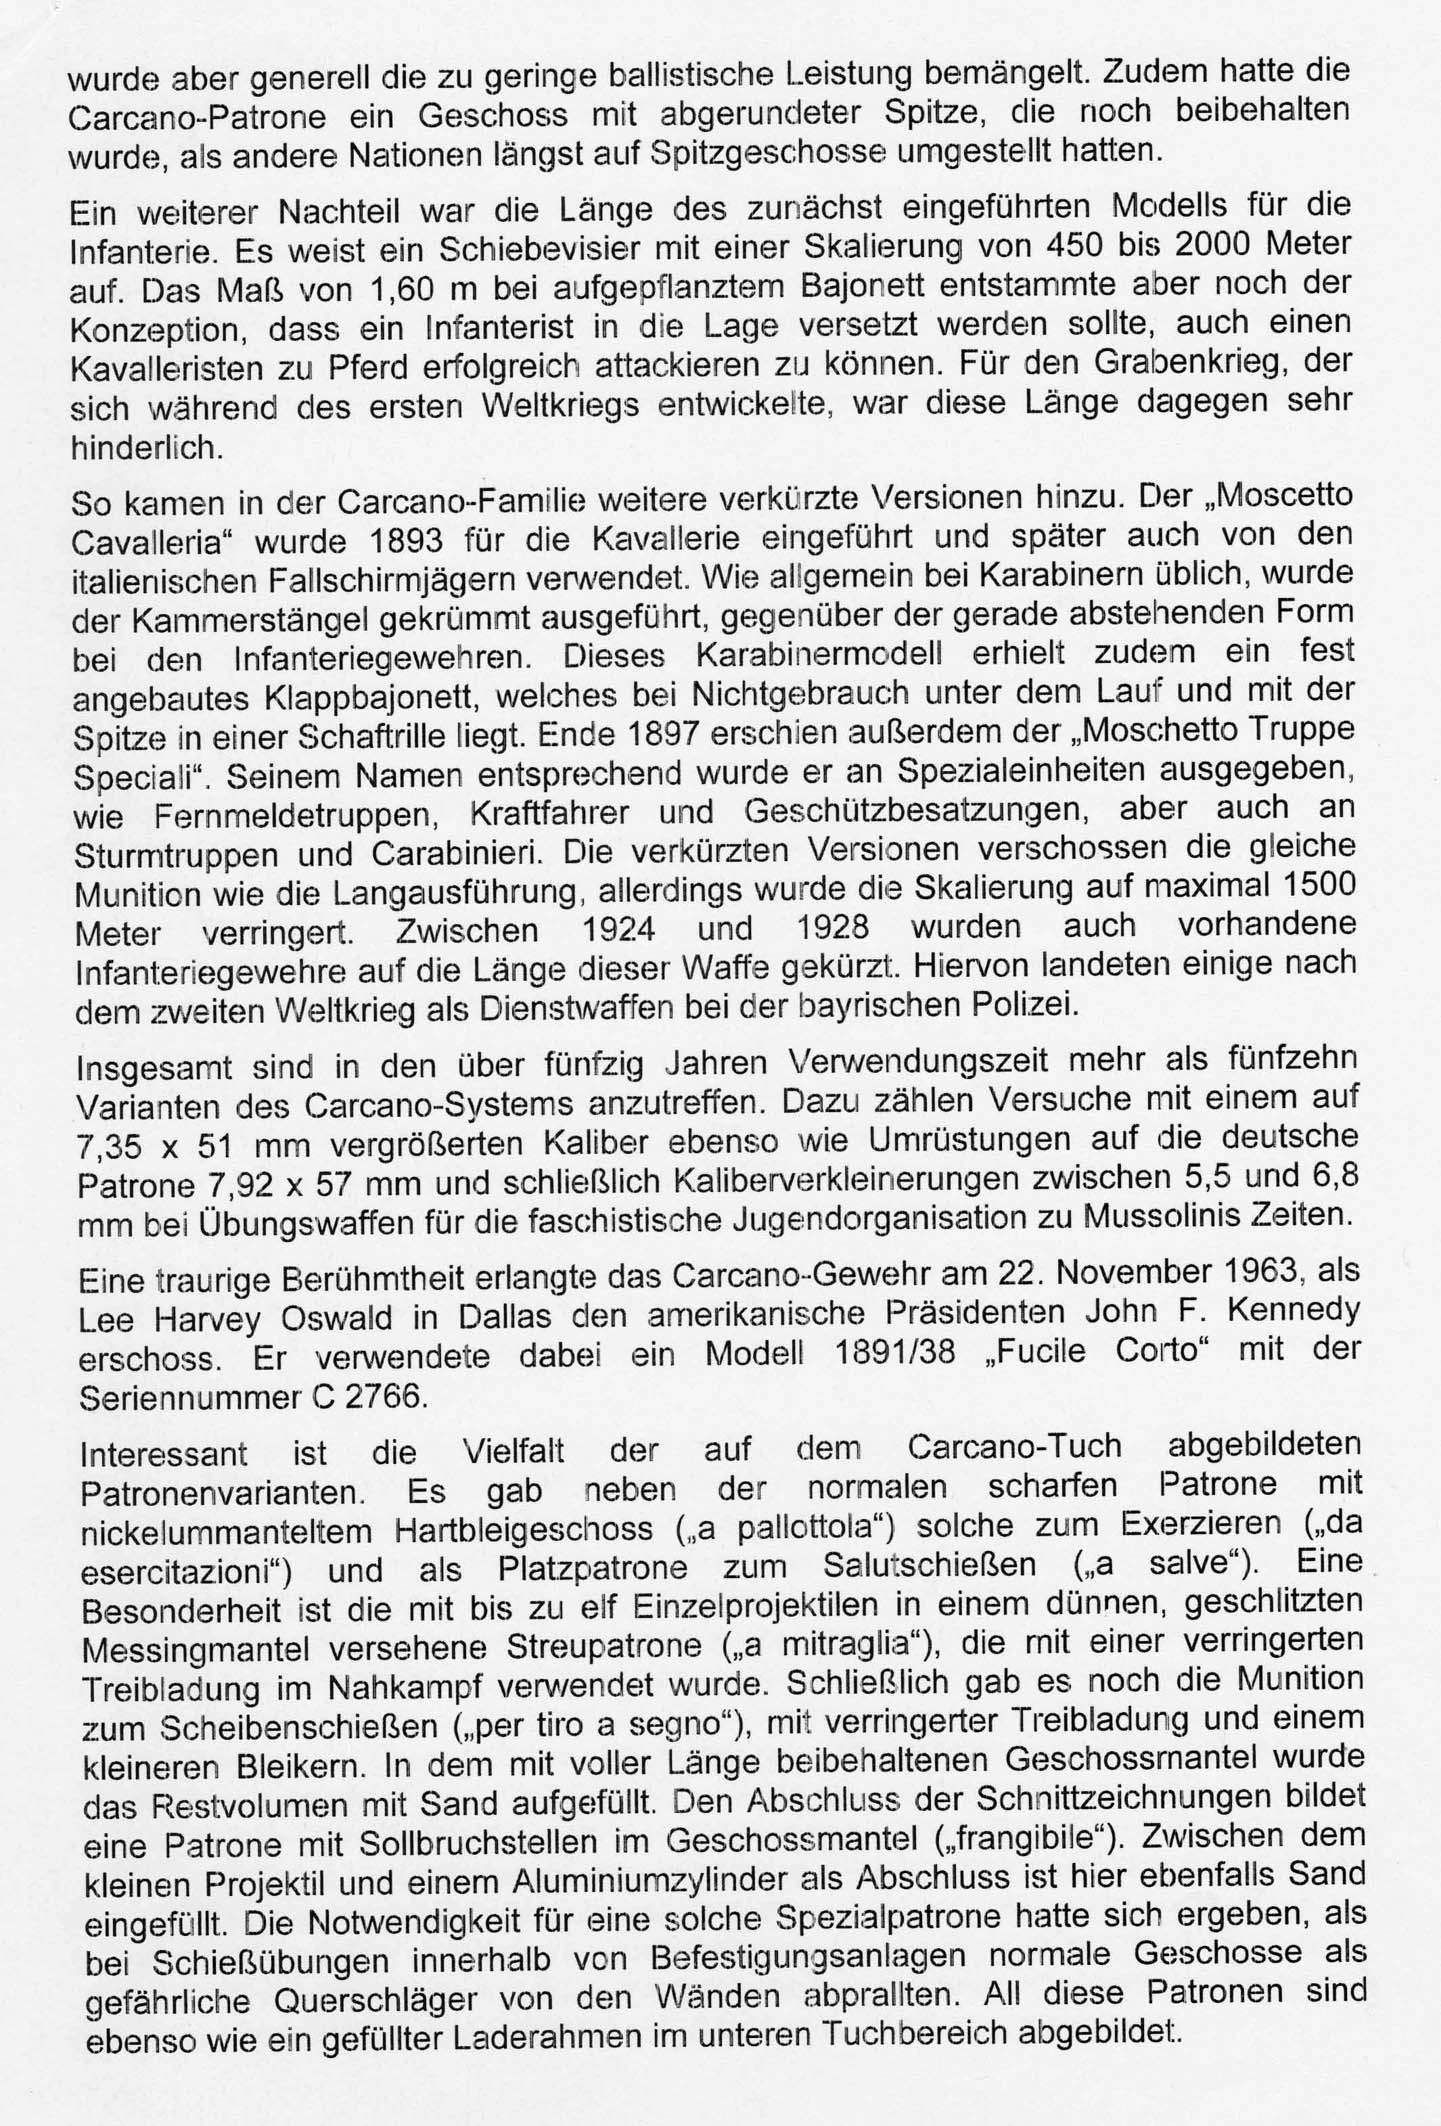
\includegraphics[width=\textwidth]{deangelifrua_3.jpg}
	\caption{}
	\label{fig:deangelifrua_3}
\end{figure}

\newpage

D'altra parte, sono state generalmente criticate le inadeguate prestazioni balistiche. Inoltre, la cartuccia Carcano che era ancora mantenuta, era un proiettile con punta arrotondata, mentre in altre nazioni da tempo si erano convertiti i proiettili. 
   Un altro svantaggio è la lunghezza del primo modello introdotto per la fanteria. Ha un mirino con una scala mobile 450-2000 metri. La lunghezza di 1,60 m con baionetta innestata, riflette ancora il concetto che un soldato dovrebbe essere in grado di attaccare anche un cavalliere per avere successo. Per la guerra di trincea, che si è sviluppata durante la Prima Guerra Mondiale, ciò è stato di molto ostacolo.
   Così si aggiunsero alla famiglia Carcano versioni ridotte. Il "Moschetto Cavalleria" è stato introdotto nel 1893 per la cavalleria e poi utilizzato dai paracadutisti italiani. Questo modello è stato anche dotato di una baionetta pieghevole, che si trova sotto la canna quando non in uso e con la punta in una scanalatura. Alla fine del 1897 apparve anche il "Moschetto Truppe Speciali". Come dice il suo nome è stato prodotto per unità speciali, come le truppe di telecomunicazioni, cannonieri e piloti, ma anche le truppe d'assalto ed i carabinieri. Le versioni accorciate sparavano le munizioni stesse di quelle lunghe, tuttavia, la portata era ridotta fino a un massimo di 1500 metri. Tra il 1924 e il 1928 i fucili di fanteria esistenti sono stati accorciati alla lunghezza di quest'arma. Di questi, alcuni finirono dopo la Seconda Guerra Mondiale usati come arma di servizio dalla polizia bavarese.
   Nel complesso, in un periodo superiore ai 50 anni furono usate più di quindici varietà di armi con sistema Carcano. Queste includono calibri allargati a 7,35 mm x 51, nonché cartucce tedesche calibro 7,92 x 57 mm e infine la riduzione dal 5,5-6,8 mm per l'organizzazione giovanile fascista al tempo di Mussolini.
   Una notorietà fu acquisita dal fucile Carcano il 22 Novembre 1963, quando Lee Harvey Oswald, a Dallas, uccise il presidente americano John F. Kennedy. Usò un modello 1891/38 "Fucile Corto" con il numero di serie C 2766.
   Interessante è la diversità delle cartucce raffigurate sul fazzoletto-Carcano. Ci sono, oltre alla normale cartuccia con copertura di nickel ("a pallottola") quelle per esercitazione ("da esercitazioni") ed una cartuccia a salve ("a salve"). Una caratteristica particolare è il massimo di undici proiettili singoli in un sottile involucro di ottone ("a mitraglia"), che è stato utilizzato con una carica propellente ridotta nelle mischie. Infine c'erano le munizioni per il tiro al bersaglio ("per Tiro a Segno"), con carica propellente ridotta e un nucleo in piombo più piccolo. Per mantenere la lunghezza completa il volume rimanente era riempito con sabbia. La conclusione dei disegni in sezione mostra una cartuccia con punti di rottura ("Frangibile"). Fra il proiettile e un piccolo cilindro di alluminio il terminale è pieno di sabbia. La necessità di tale una speciale cartuccia si era evidenziata, dal momento che nel tiro al bersaglio con normali proiettili essi rimbalzavano pericolosamente colpendo le pareti. Queste cartucce sono mostrate nell'area inferiore del fazzoletto.
Sui fazzoletti italiani si possono anche trovare le immagini e le spiegazioni delle varie formazioni di fanteria.

\newpage

\begin{figure}[h]
	\centering
		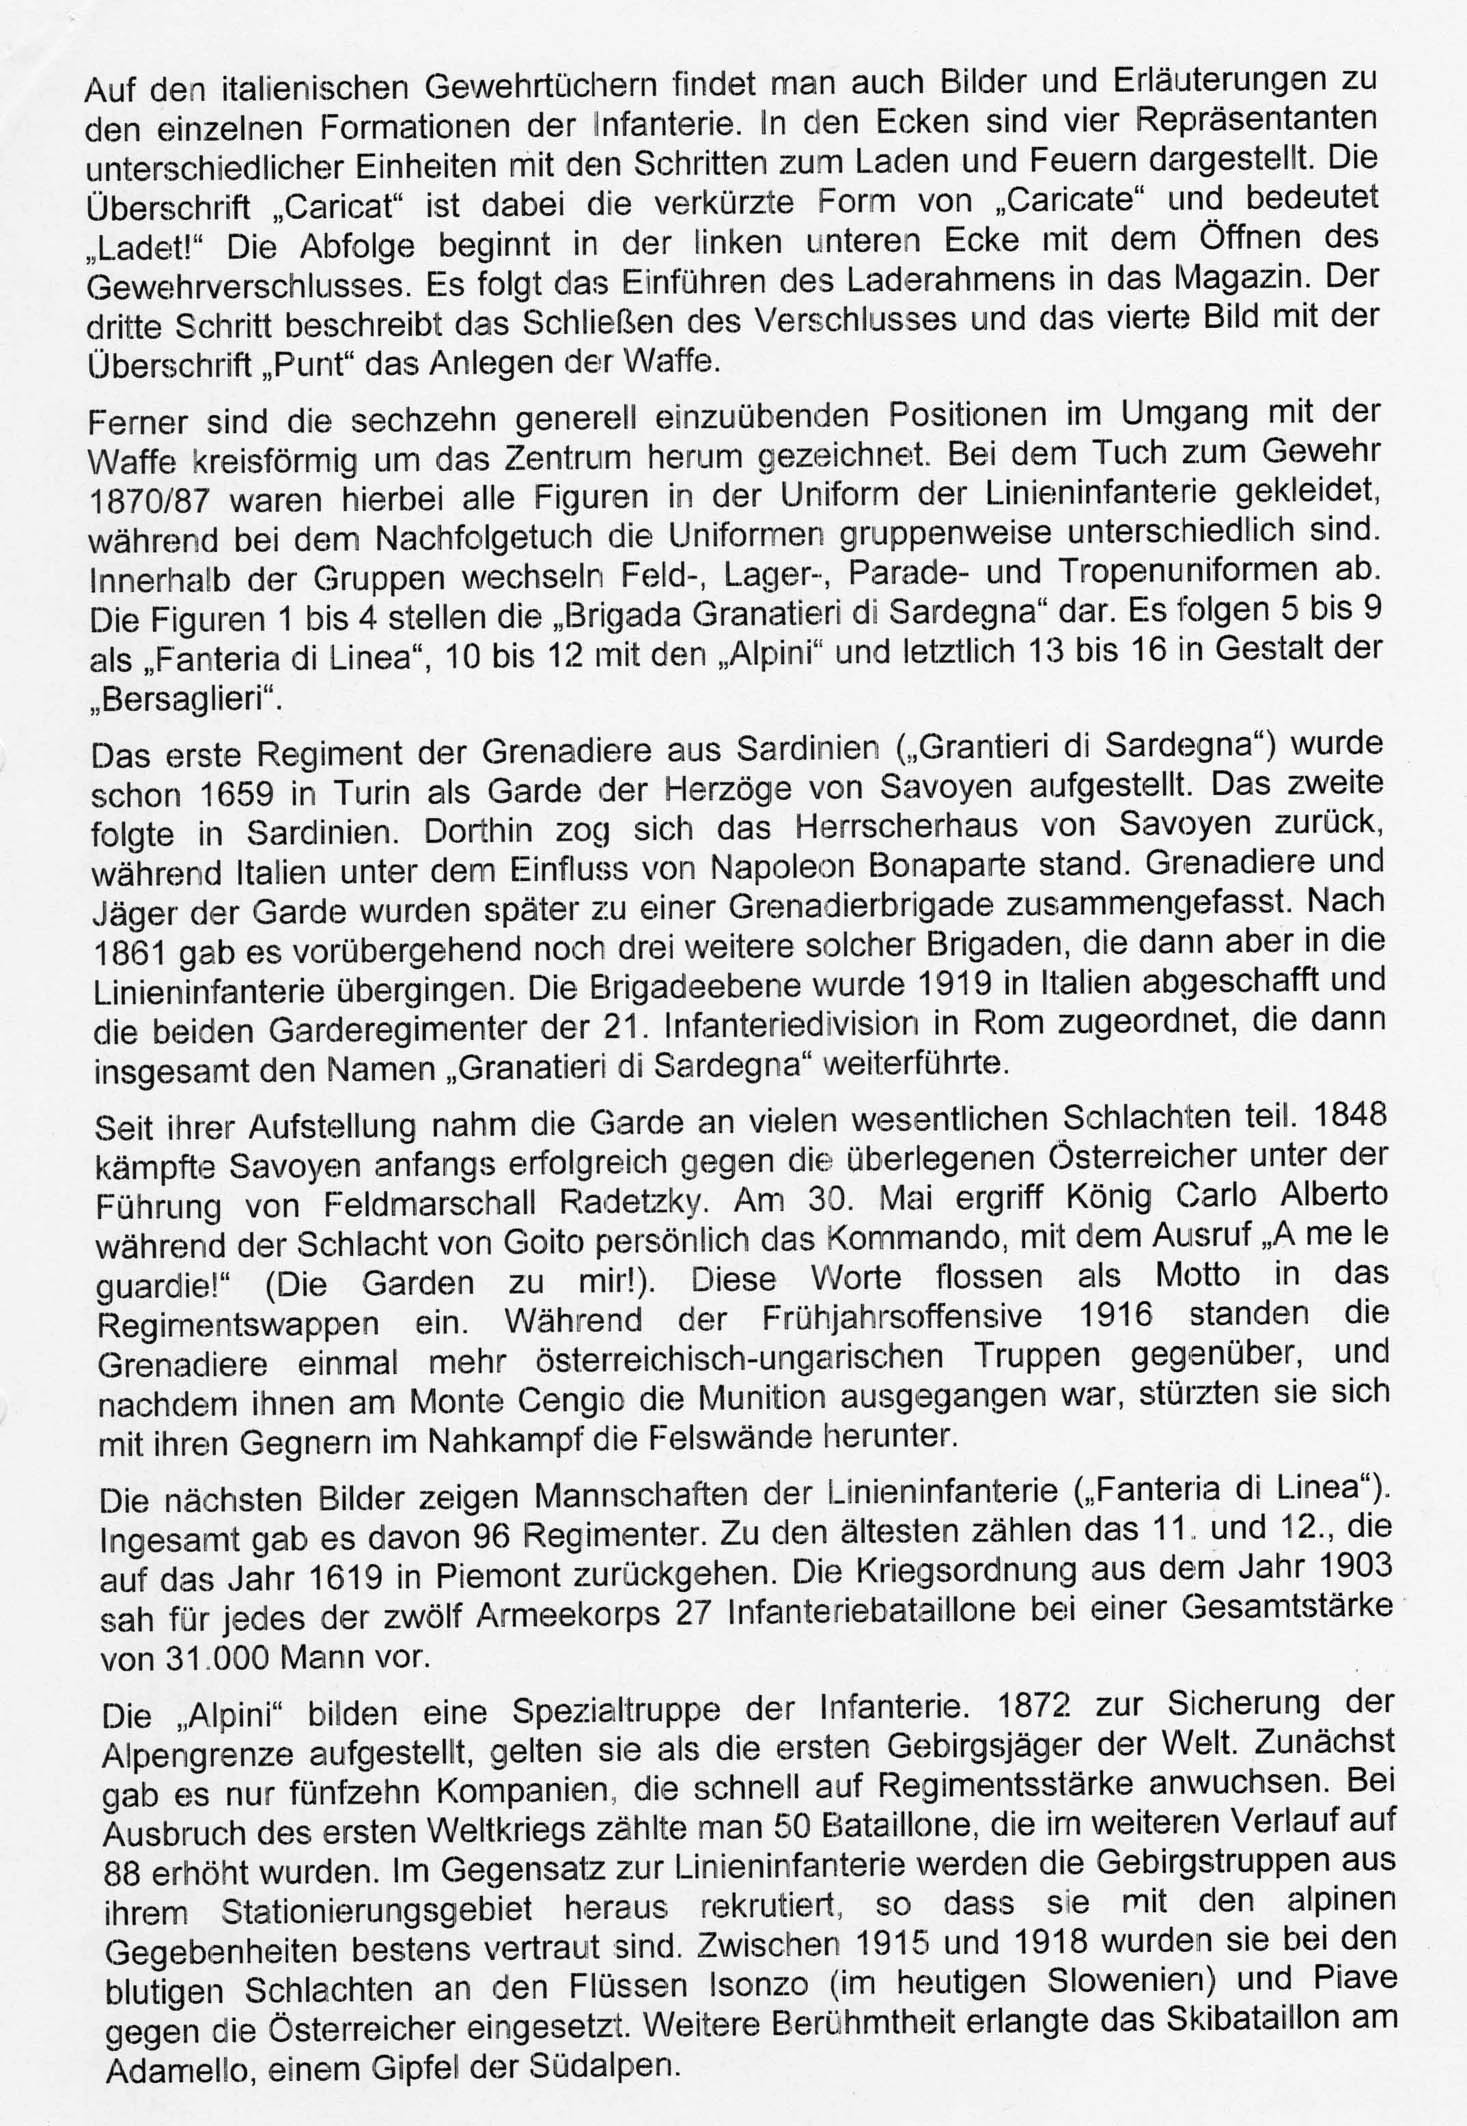
\includegraphics[width=\textwidth]{deangelifrua_4.jpg}
	\caption{}
	\label{fig:deangelifrua_4}
\end{figure}

\newpage

Negli angoli stanno quattro rappresentanti di diverse unità che mostrano i passaggi per il caricamento ed il fuoco. La scritta "caricat" è la forma abbreviata di "caricate" e significa "Carica!" La sequenza inizia nell'angolo in basso a sinistra con l'apertura della caricatore. Ne consegue l'introduzione dei proiettili nel caricatore. Il terzo passo descrive la chiusura e la quarta immagine con la scritta"punt" nella parte superiore il puntamento dell'arma.
   Inoltre, sono illustrate le sedici posizioni generali uso dell'arma in un cerchio intorno al centro. Nel fazzoletto per fucile 1870/87 le figure sono tutte in uniforme della fanteria di linea, mentre nei fazzoletti successivi i gruppi di divise sono diversi. All'interno dei gruppi le uniformi sono da campo, da deposito, da parata e coloniali. Le figure da 1 a 4 rappresentano la "Brigata Granatieri di Sardegna" A seguire da 5 a 9 la "Fanteria di Linea", da 10 a 12 gli "Alpini" e infine da 13 a 16 i "Bersaglieri".
II primo reggimento dei Granatieri di Sardegna  fu istituito nel 1659 a Torino come guardia dei duchi di Savoia. 
   II secondo seguì in Sardegna. Ci si era ritirata la casa regnante dei Savoia, mentre l'Italia era sotto l'influenza di Napoleone Bonaparte. I Granatieri della Guardia e i Cacciatori sono stati successivamente raccolti in una brigata. Dopo il 1861 ci furono altre tre brigate, ma poi confluirono nella fanteria di linea. La brigata è stata abolita nel 1919 in Italia e i due reggimenti Guardie della 21 Divisione di fanteria, furono assegnati a Roma, che poi hanno portato il nome di "Granatieri di Sardegna".
   Fin dalla sua costituzione, la Guardia ha partecipato a molte battaglie importanti. Nel 1848 i Savoia inizialmente hanno combattuto con successo contro gli austriaci comandati dal maresciallo Radetzky. Il 30 Maggio re Carlo Albèrto prese il comando personale durante la battaglia di Goito, con l'esclamazione "A me le Guardie!". Queste parole sono state incorporate nel motto del reggimento. Durante l'offensiva di primavera del 1916 i granatieri hanno resistito contro le truppe austro-ungariche, e dopo aver esaurito le munizioni a Monte Cengio, si buttavano giù con i loro nemici in combattimento ravvicinato, dalle pareti di roccia.
   Le immagini successive mostrano di squadre di fanteria di linea ("Fanteria di Linea"). Complessivamente ci sono stati 96 reggimenti. Fra i più antichi sono l'11 e il 12, che risalgono al 1619, in Piemonte. Le ordinanze del 1903 per ciascuno delle dodici corpi di armata dell'esercito, prevedevano 27 battaglioni di fanteria con una forza totale di 31.000 uomini. 
   Gli "Alpini" formano una speciale forza di fanteria. Istituiti nel 1872 per assicurare la frontiera alpina, sono considerati i primi cacciatori di montagna del mondo. Inizialmente c'erano solo quindici compagnie, che crebbero rapidamente alla forza di un reggimento. Allo scoppio della seconda guerra mondiale c'erano 50 battaglioni, che sono stati aumentati a 88. In contrasto con la fanteria di linea, le truppe di fanteria di montagna sono reclutate dalla loro zona di provenienza in modo a essere al corrente delle condizioni alpine. Tra il 1915 e il 1918 furono impiegati in sanguinose battaglie sul fiume Isonzo (oggi in Slovenia) e sul Piave contro gli austriaci. Ebbero fama ulteriormente i battaglioni da sci dell'Adamello, una cima delle Alpi Meridionali.
   
\newpage

\begin{figure}[h]
	\centering
		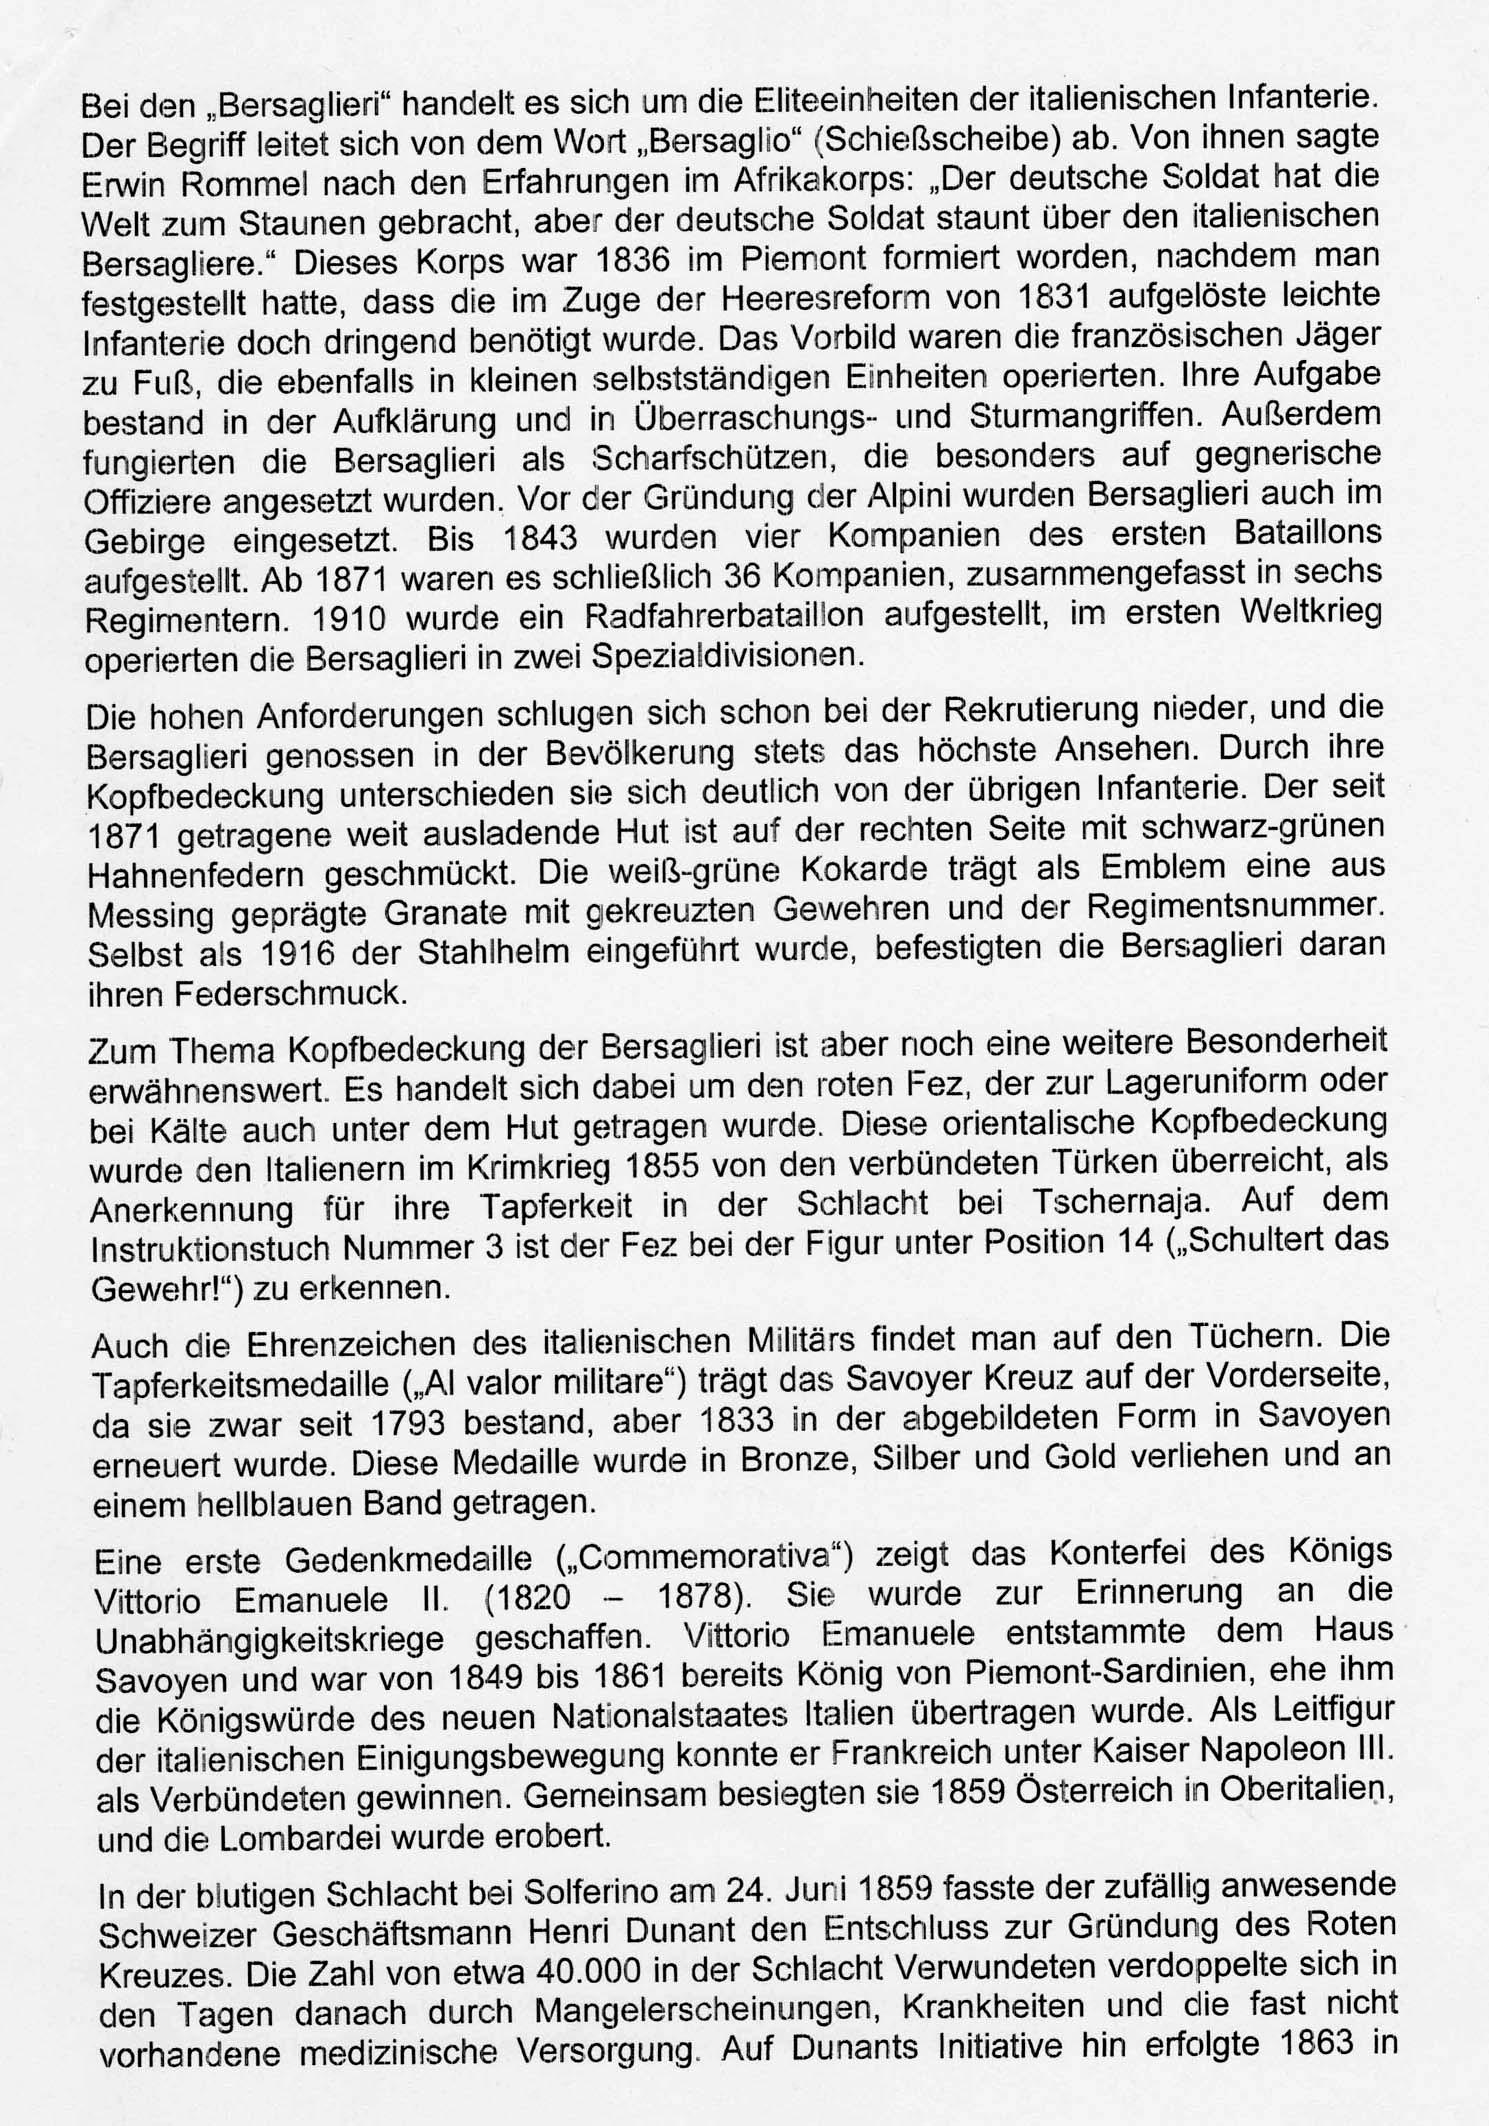
\includegraphics[width=\textwidth]{deangelifrua_5.jpg}
	\caption{}
	\label{fig:deangelifrua_5}
\end{figure}

I "Bersaglieri" sono le unità d'elite della fanteria italiana. Il termine deriva dalla parola "Bersaglio". Erwin Rommel di loro ha detto dopo l'esperienza nell'Afrika korps: "II soldato tedesco è ammirato nel mondo, ma il soldato tedesco ammirò il Bersagliere italiano". Questo corpo si era formato nei 1836 in Piemonte, dopo la riforma dell'esercito del 1831 come di fanteria leggera e rapida. Il modello era il cacciatore francese a piedi, che operava in piccole unità indipendenti. Il loro compito era la perlustrazione, la sorpresa e l'assalto. Operando i bersaglieri come tiratori, che erano particolarmente considerati dagli ufficiali nemici. Prima della fondazione degli Alpini, i Bersaglieri sono stati utilizzati anche in montagna. Fino al 1843, furono schierate quattro compagnie del Primo Battaglione. Dal 1871, ci sono state 36 compagnie raggruppate in sei reggimenti. Nel 1910 è stato allestito un battaglione ciclista. Nella prima guerra mondiale, i bersaglieri operavano in due divisioni speciali.
   I severi requisiti si riflettevano nel reclutamento, e i bersaglieri hanno sempre goduto della massima reputazione da parte della popolazione. Con i loro cappelli, differivano significativamente dal resto della fanteria. Il cappello indossato dal 1871, è decorato sul lato destro con piume di gallo cedrone. La coccarda verde e bianco reca come un distintivo di ottone sbalzato fucili e granate con il numero del reggimento. Anche sull'elmo d'acciaio 1916 i bersaglieri misero le loro piume. A proposito del copricapo dei Bersaglieri vi è ancora da fare un'altra menzione speciale. E 'il fez rosso, che è stato portato nell'uniforme al campo, o quando fa freddo anche sotto il cappello. Questo copricapo orientale fu donato agli italiani nella guerra di Crimea nel 1855, dai turchi alleati, in riconoscimento del loro coraggio nella battaglia di Chernaya. Sul fazzoletto di istruzioni n. 3 il Fez figura al punto 14 ("in spalla il suo fucile!").
   Anche le decorazioni dei militari italiani si trovano sui fazzoletti. La Medaglia ("al valor militare") che porta sulla parte anteriore la croce di Savoia, esisteva sin dal 1793, ma è stata rinnovata nel 1833. Questa medaglia è stata assegnata in bronzo, argento e oro e indossata con un nastro azzurro.
   Una prima medaglia commemorativa  mostra l'immagine di Re Vittorio Emanuele II (1820 - 1878). E 'stata creata per commemorare le guerre di indipendenza. Vittorio Emanuele veniva dalla Casa di Savoia ed era già re di Piemonte-Sardegna dal 1849 al 1861, prima di diventare il Re del nuovo stato nazionale italiano. Come guida del movimento di unificazione italiana, è stato alleato con la Francia sotto l'imperatore Napoleone III. insieme hanno sconfitto l'Austria nel 1859 nel nord Italia, e la Lombardia è stata conquistata.
   
\newpage

Nella sanguinosa battaglia di Solferino, il 24 Giugno 1859 l'imprenditore svizzero Henri Dunant prese la decisione di fondare la Croce Rossa. Il numero di circa 40.000 feriti in battaglia raddoppiò nei giorni seguenti per malattie, e quasi nessuna cura medica a disposizione. Per iniziativa di Dunant a Ginevra nel 1863 fu istituito il "Comitato internazionale di soccorso ai feriti in battaglia".

\begin{figure}[h]
	\centering
		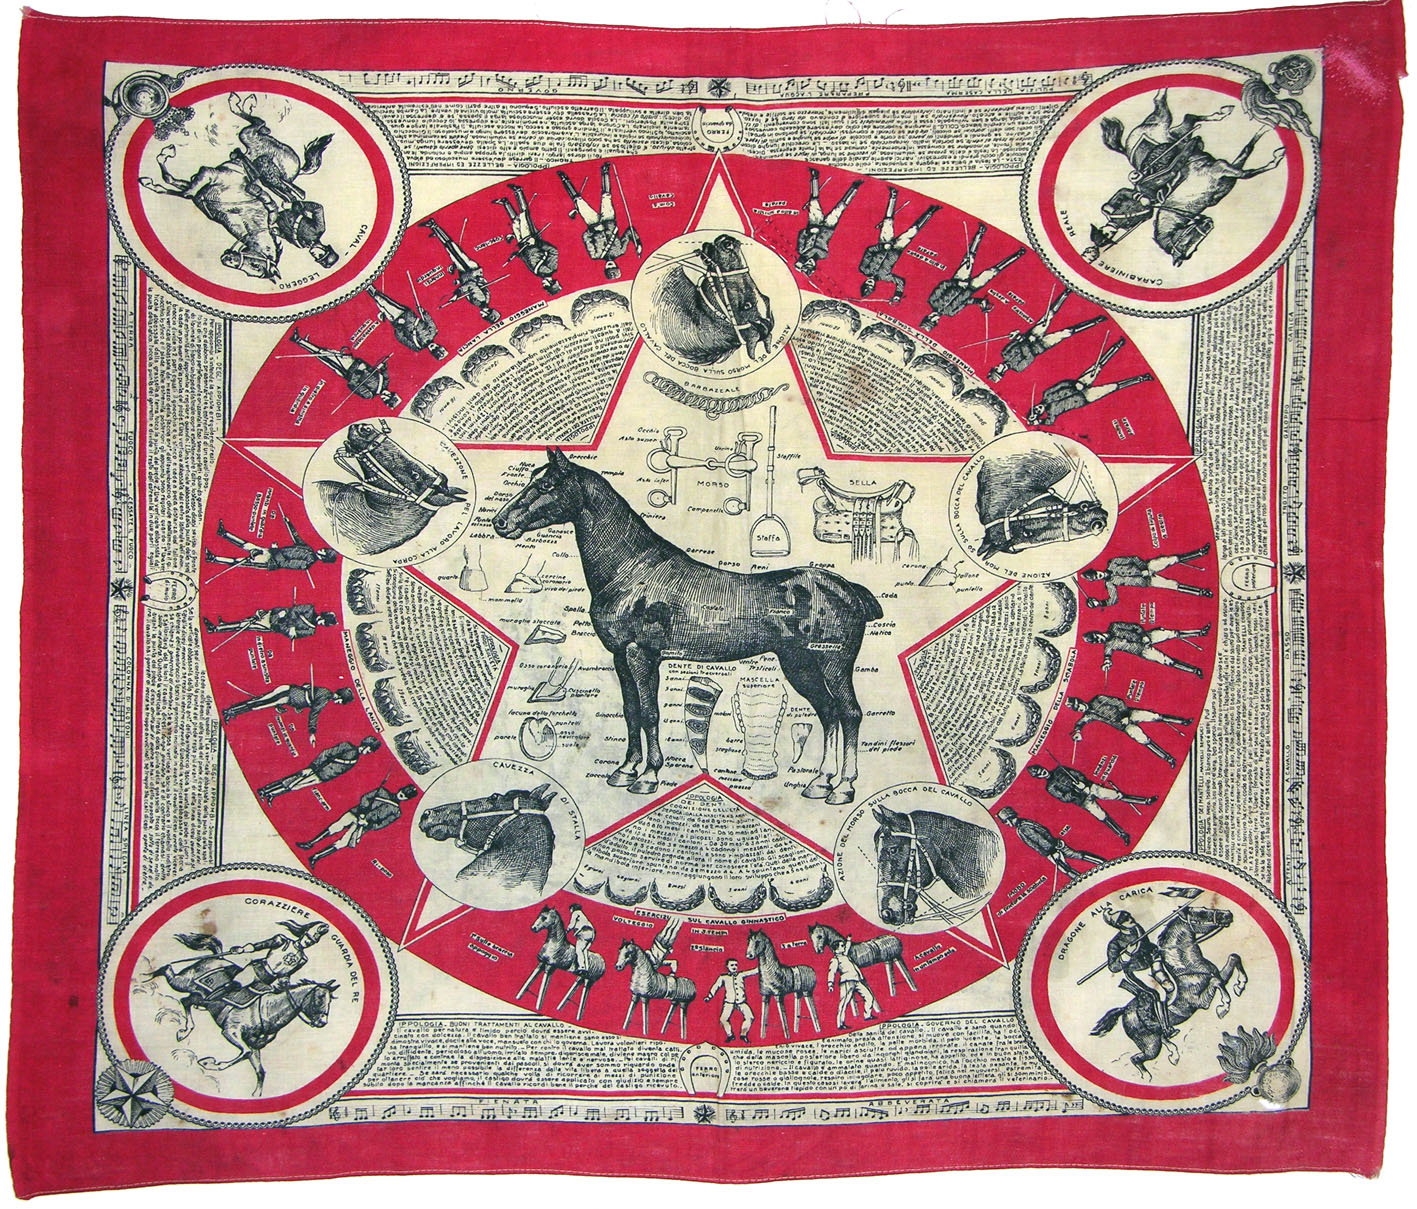
\includegraphics[width=\textwidth]{fazzoletto4_cavalleria.jpg}
	\caption{Fazzoletto militare italiano n°4 per Cavalleria. Stamperia E. De Angeli \&Co. – Milano}
	\label{fig:fazzoletto4_cavalleria}
\end{figure}

\newpage

\begin{figure}[h]
	\centering
		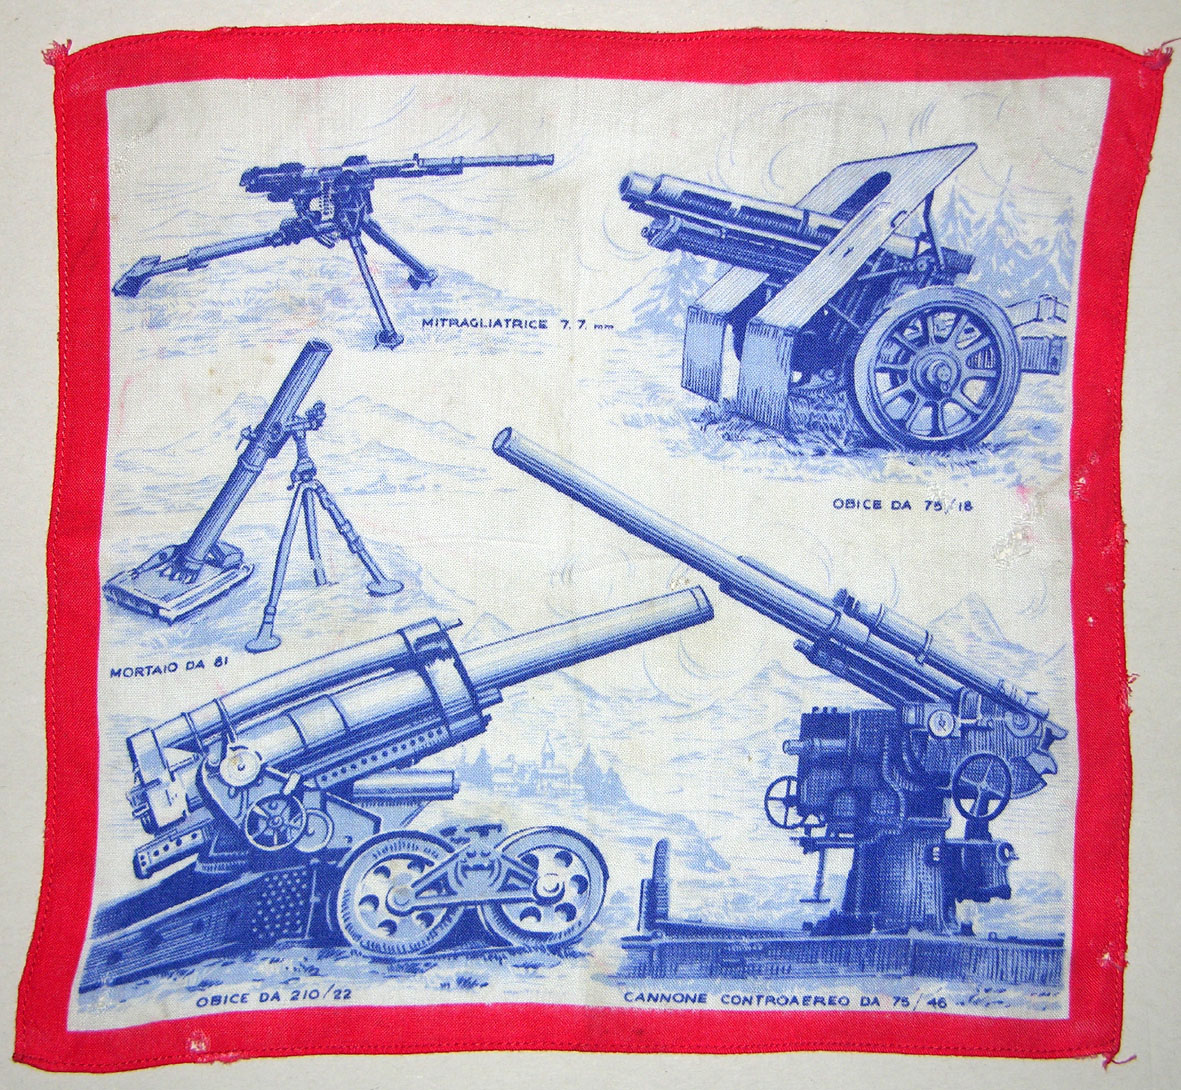
\includegraphics[width=\textwidth]{fazzoletto_armipesanti.jpg}
	\caption{Fazzoletto per armi pesanti}
	\label{fig:fazzoletto_armipesanti}
\end{figure}

\newpage

\begin{figure}[h]
	\centering
		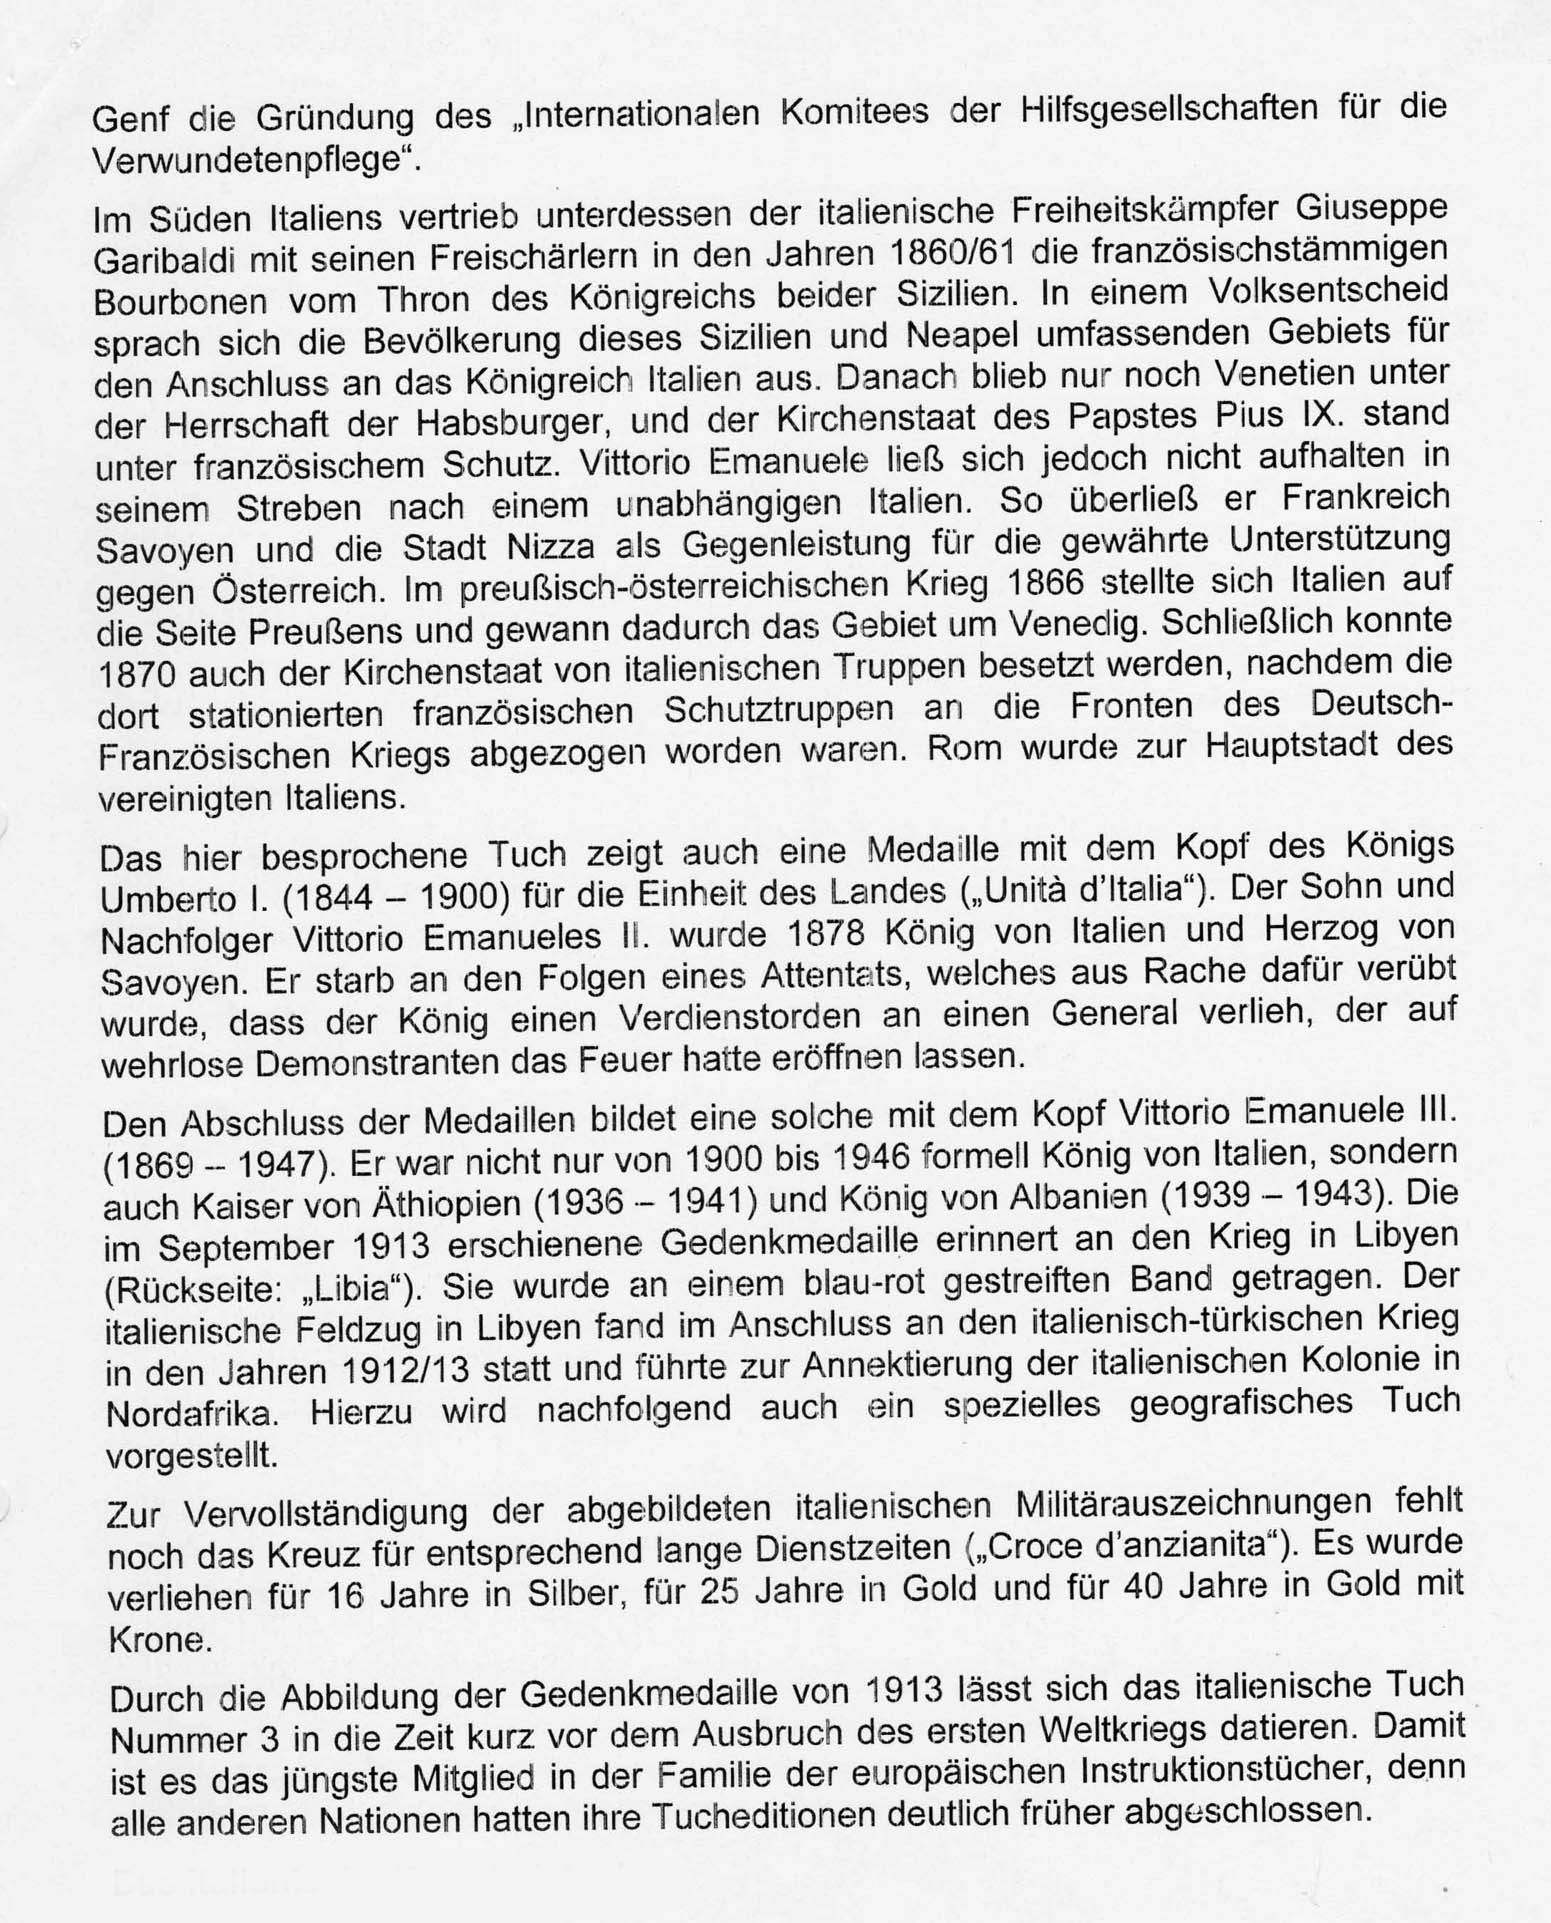
\includegraphics[width=\textwidth]{deangelifrua_6.jpg}
	\caption{}
	\label{fig:deangelifrua_6}
\end{figure}

\newpage

Nel sud Italia, nei frattempo, l'italiano Giuseppe Garibaldi, ha scacciato con i suoi guerriglieri nel 1860/61 i Borboni francesi di nascita dal trono del Regno delle Due Sicilie. in un plebiscito, il popolo di questa vasta area della Sicilia e di Napoli si espresse per l'unione al Regno d'Italia. Da allora in poi solo il Veneto rimase sotto il dominio degli Asburgo, e Io Stato della Chiesa di Papa Pio IX era sotto la protezione francese. Vittorio Emanuele, però, non si fermò nella lotta per l'indipendenza d'Italia. Così lasciò la città di Nizza e la Savoia alla Francia in cambio del sostegno avuto contro l'Austria. Nella guerra austro-prussiana nel 1866 l'Italia si schierò con la Prussia e, quindi, ottenne la zona intorno a Venezia. Infine, nel 1870 anche lo Stato Pontificio è stato occupato dalle truppe italiane, di stanza là dopo che le truppe francesi erano state ritirate per proteggere il fronte della guerra franco-tedesca. Roma divenne capitale dell'Italia unita.
   II fazzoletto riporta anche una medaglia con la effigie del re Umberto I (1844 - 1900) per l'unità del paese ("Unità d'Italia"). Il figlio e successore di Vittorio Emanuele II, re d'Italia nel 1878 e duca di Savoia. Morì a causa di un attentato che fu perpetrato per colpire il re che aveva decorato un generale che aveva aperto il fuoco contro manifestanti disarmati.
   La conclusione delle medaglie mostra una effigie di Vittorio Emanuele III. (1869 - 1947). Non fu solo dal 1900 al 1946 Re d'Italia, ma anche Imperatore d'Etiopia (1936 - 1941) e Re d'Albania (1939 - 1943). La medaglia commemorativa è stato coniata nel settembre 1913 e ricorda la guerra di Libia (retro: "Libia"). E dotata di un nastro blu e rosso a strisce. In seguito alla campagna italiana in Libia in seguito ha avuto luogo la guerra italo-turca nel 1912/13, che portò alla annessione della colonia italiana in Africa del Nord. A tal fine, fu presentato anche uno speciale fazzoletto geografico.
   Per completare i riconoscimenti ai militari italiani fù coniata la croce per lunghi periodi di servizio ("Croce d'anzianità"). Erano premiati in argento per 16 anni, in oro per 25 anni e in oro con una corona per 40 anni.
   L'illustrazione della medaglia commemorativa del 1913, permette di datare il fazzoletto italiano n° 3 al periodo di poco precedente lo scoppio della prima guerra mondiale. E' il più giovane membro della famiglia di fazzoletti di istruzione europea, perché tutte le altre nazioni avevano completato la loro edizione di fazzoletti molto prima.
   
\newpage

\begin{figure}[h]
	\centering
		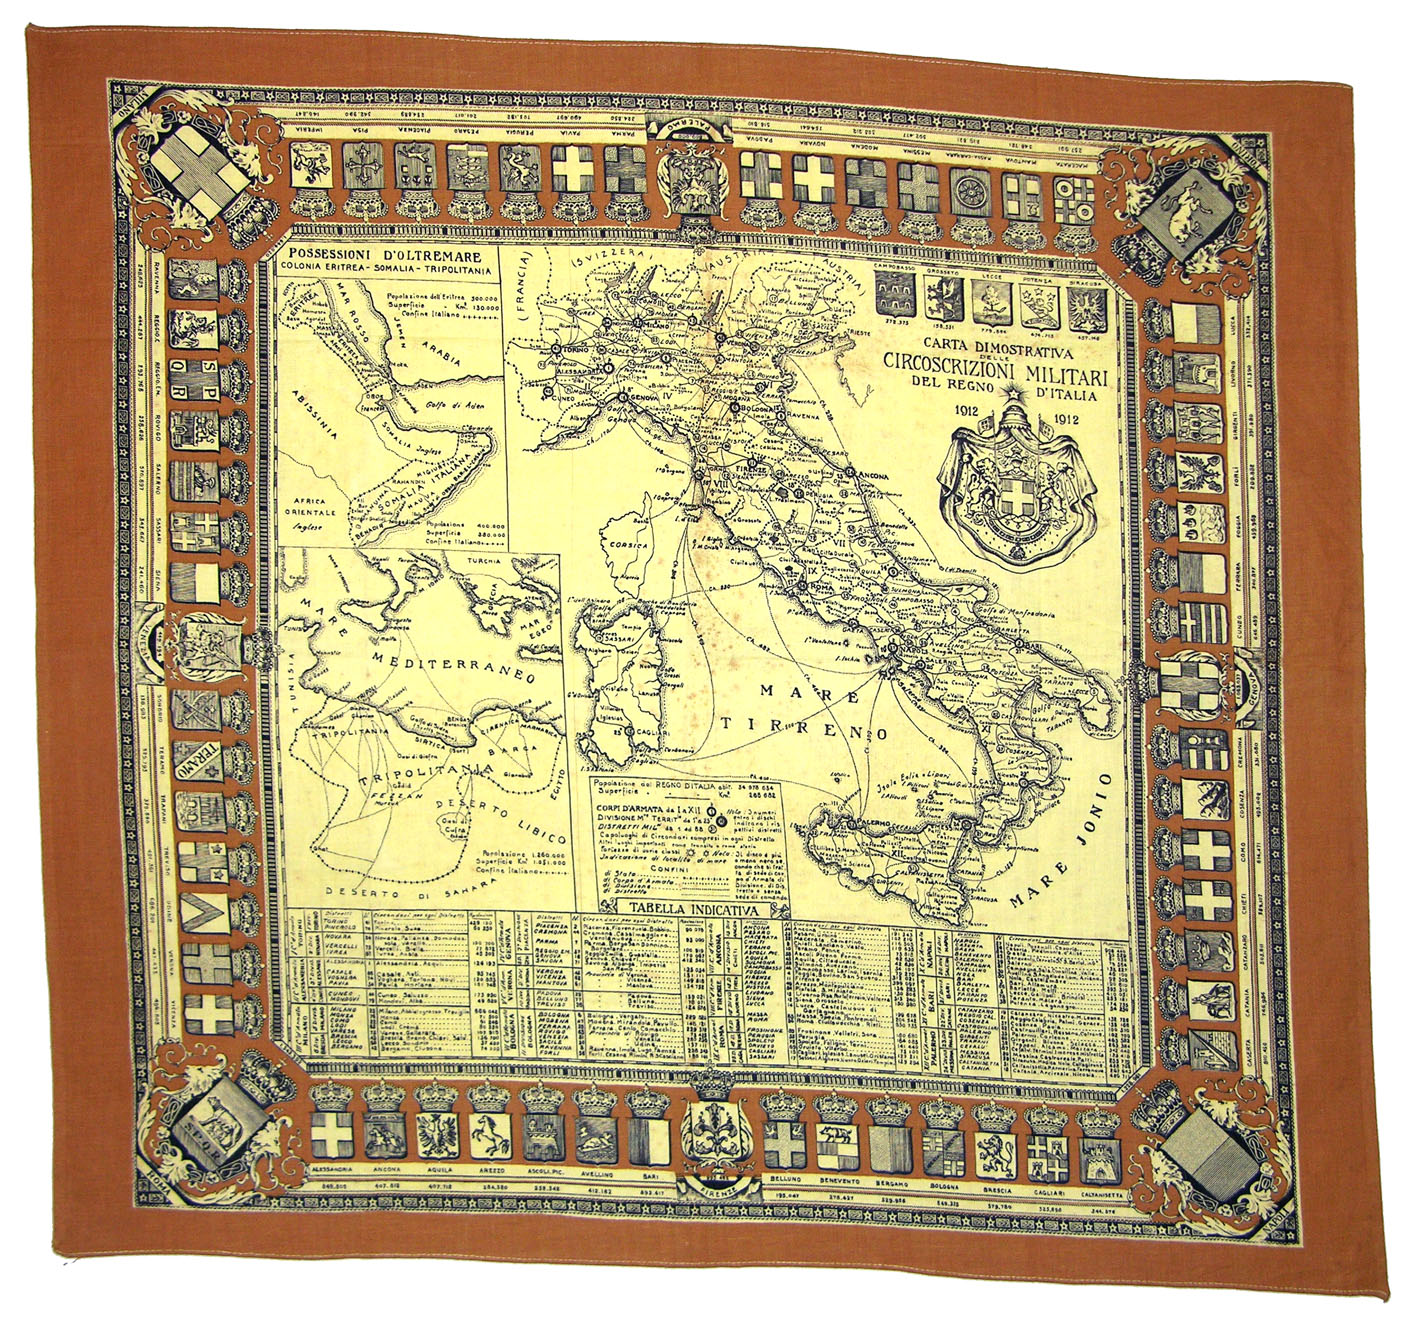
\includegraphics[width=\textwidth]{fazzoletto5_cartaitalia.jpg}
	\caption{Carta d’Italia 1912 Fazzoletto militare italiano n°5 Stamperia E. De Angeli Frua – Milano}
	\label{fig:fazzoletto5_cartaitalia}
\end{figure}

\newpage

\begin{figure}[h]
	\centering
		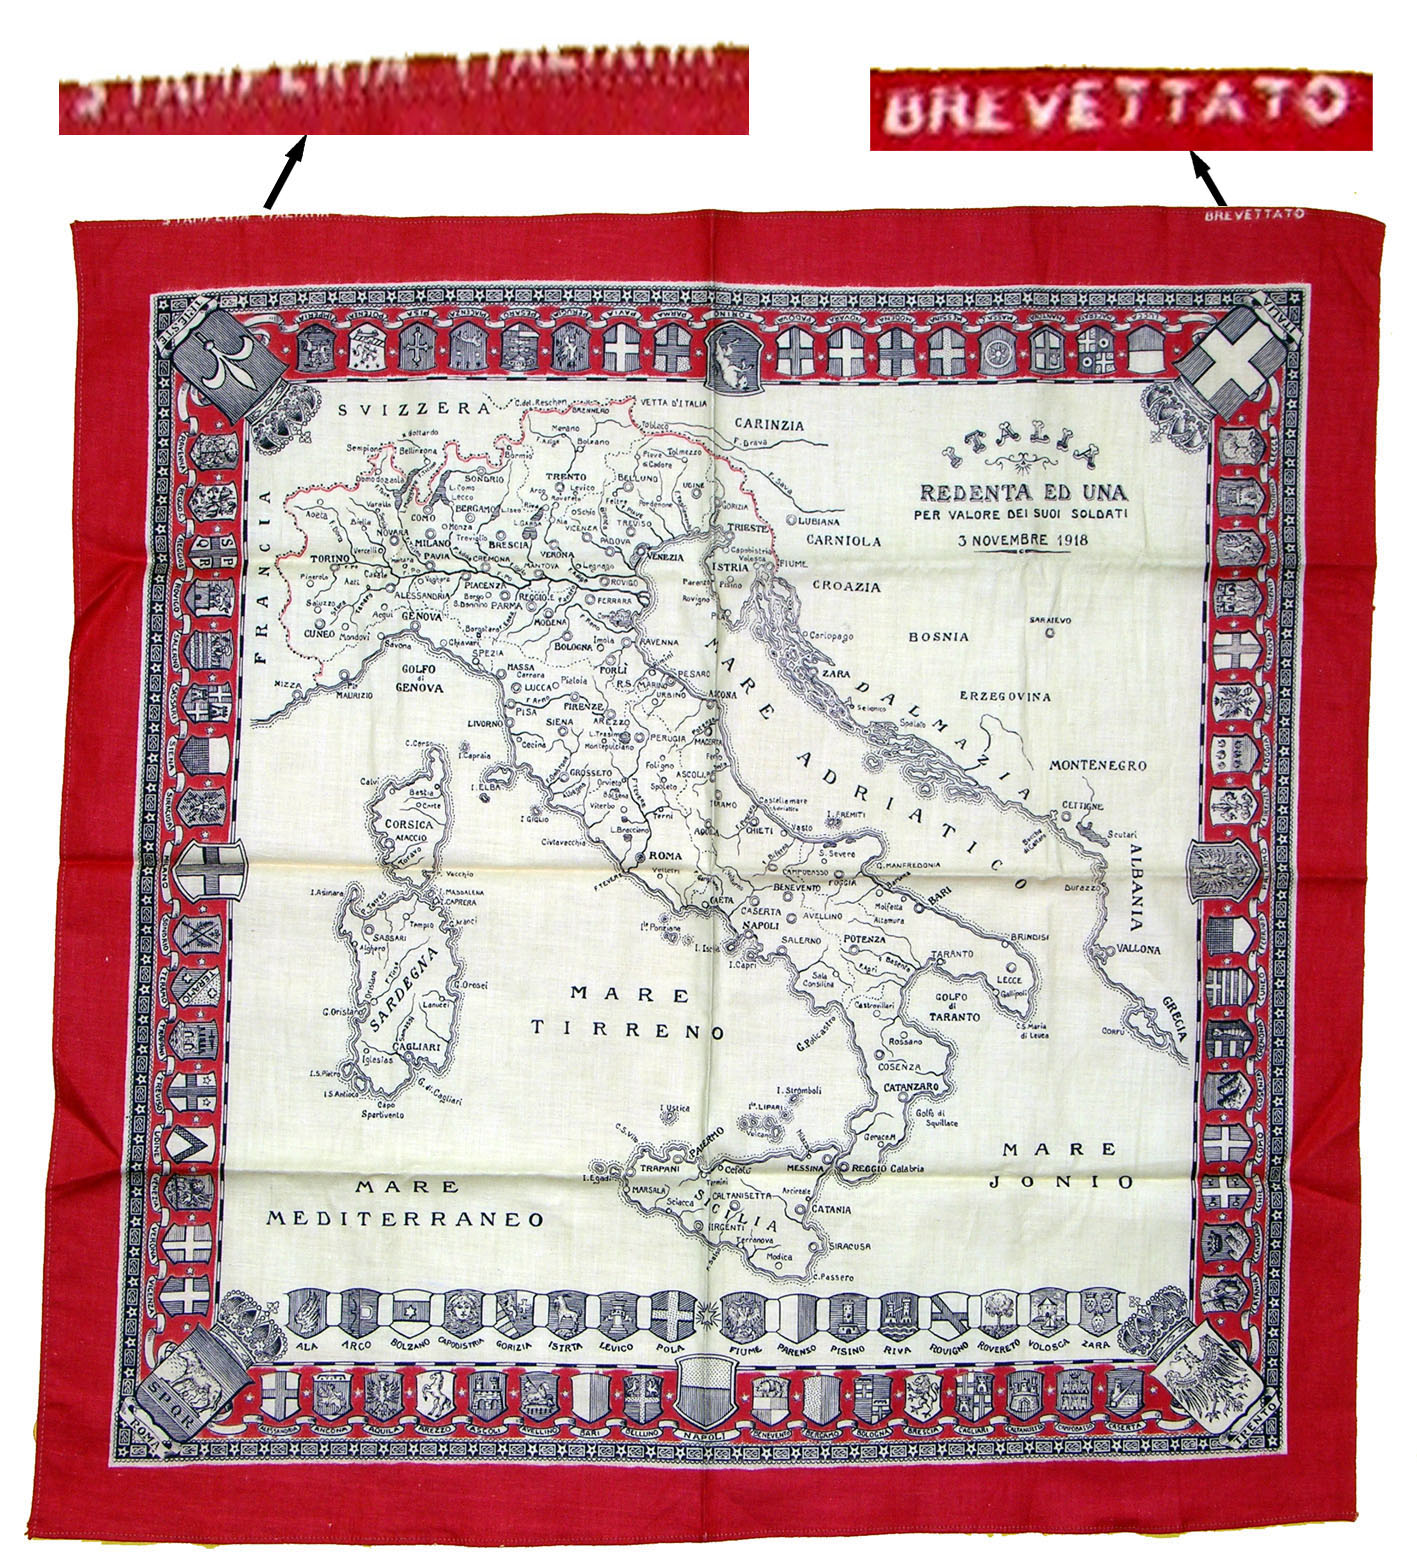
\includegraphics[width=\textwidth]{fazzoletto6_cartaitalia.jpg}
	\caption{Carta d’Italia 1918 Fazzoletto militare italiano n°6 Stamperia E. De Angeli Frua – Milano}
	\label{fig:fazzoletto6_cartaitalia}
\end{figure}

\newpage

\begin{figure}[h]
	\centering
		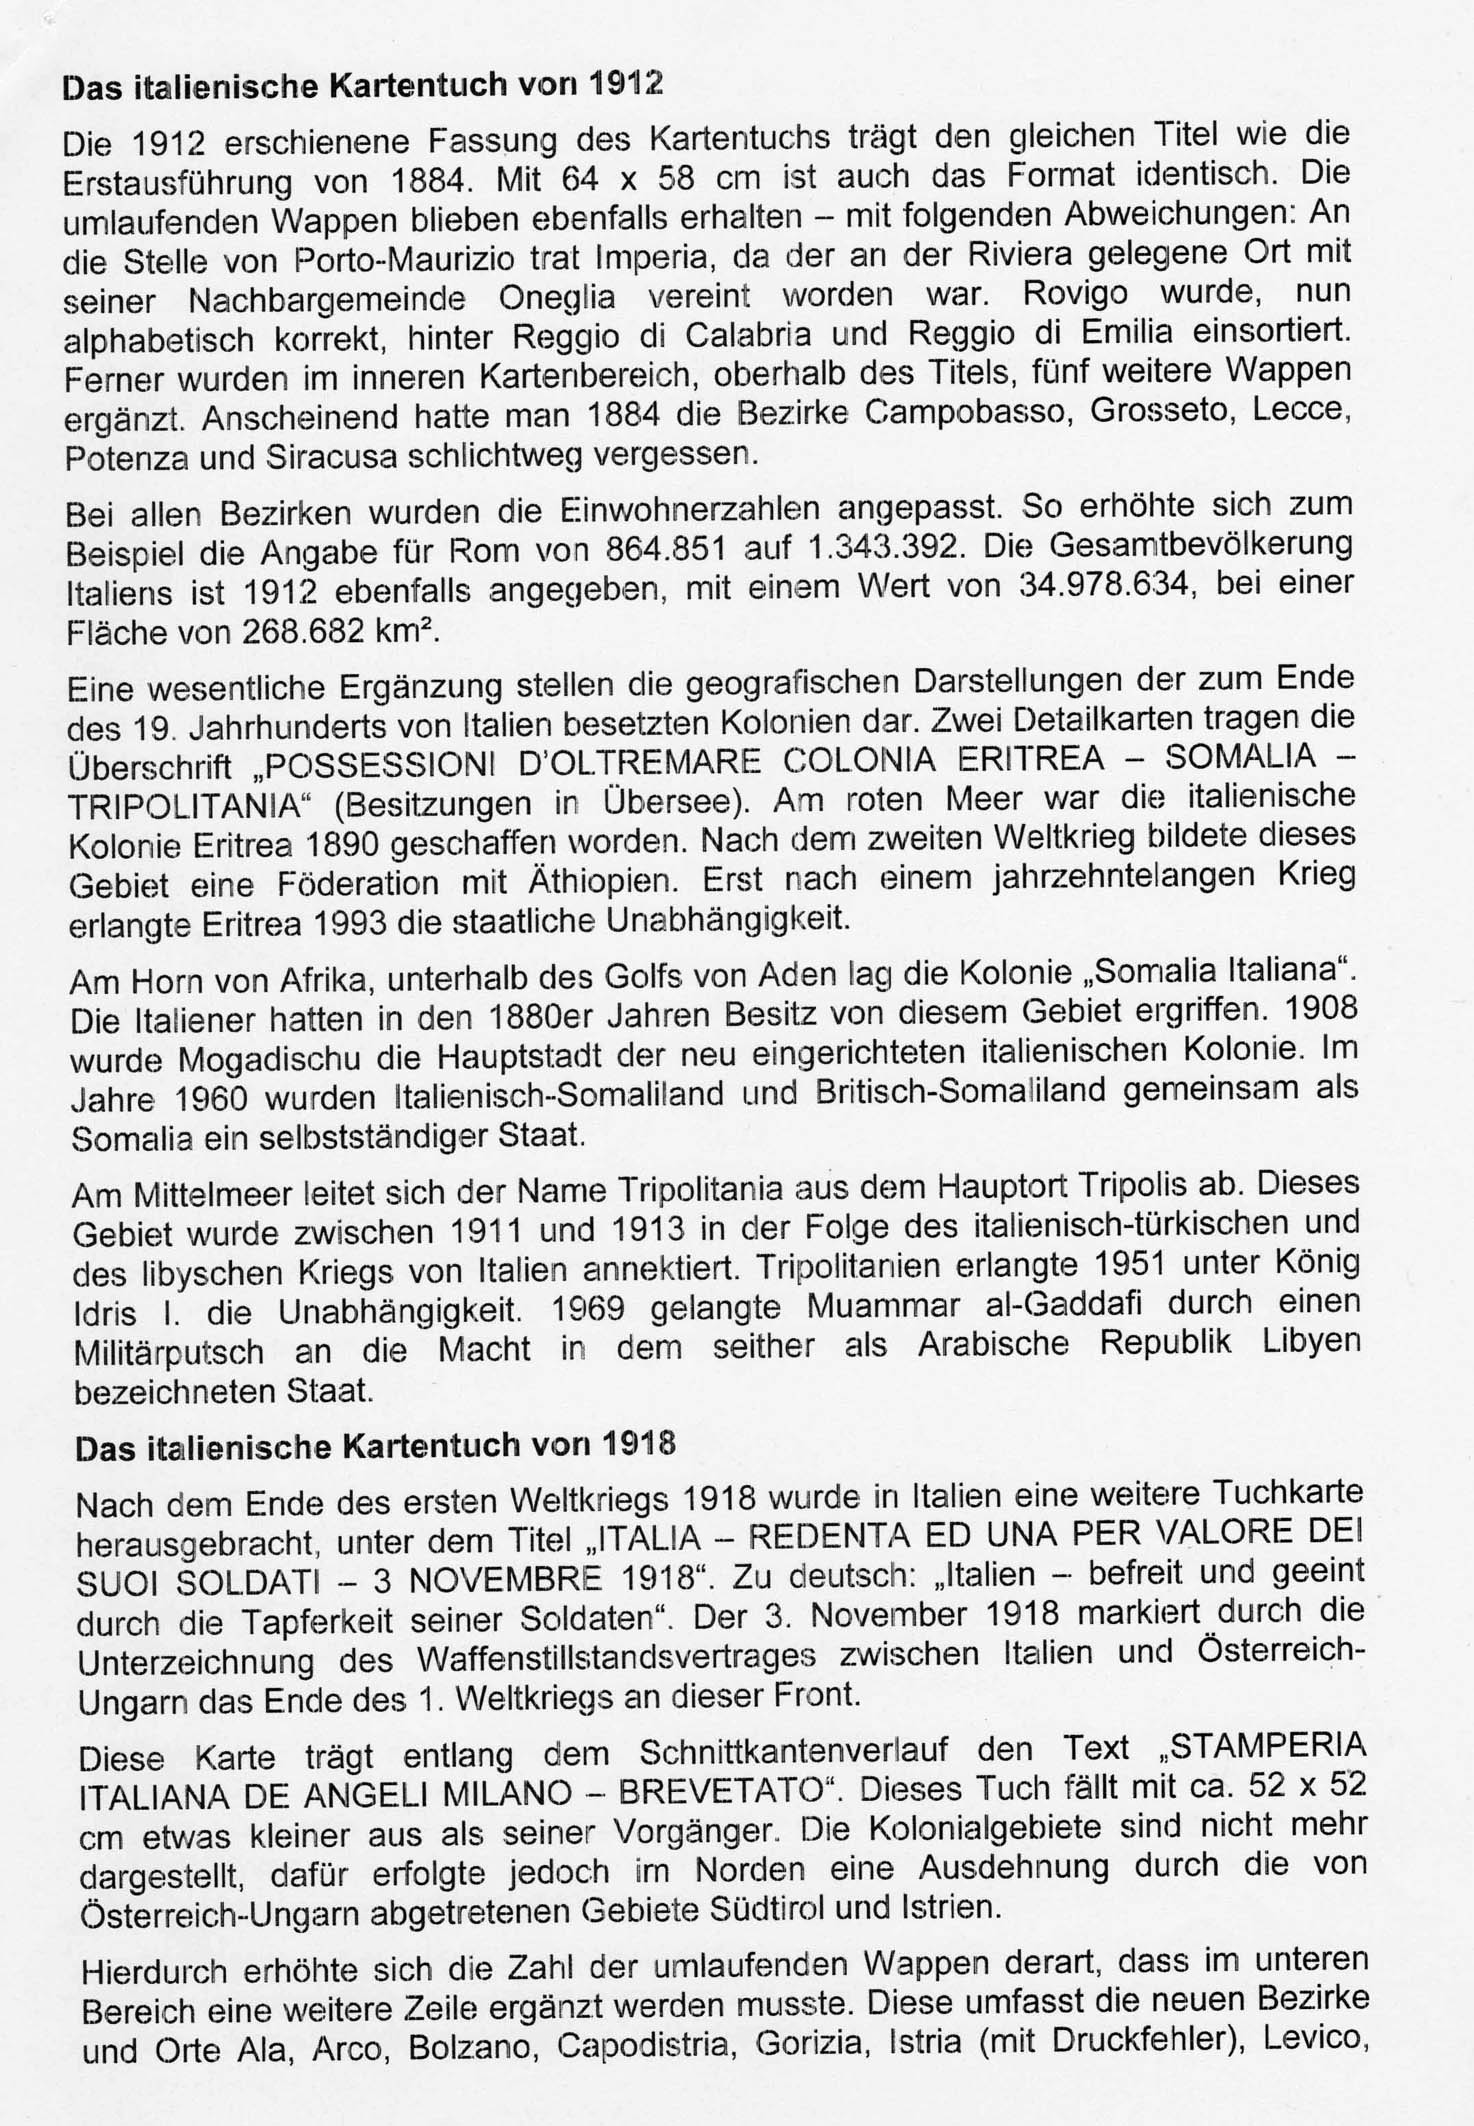
\includegraphics[width=\textwidth]{deangelifrua_7.jpg}
	\caption{}
	\label{fig:deangelifrua_7}
\end{figure}

\newpage

Il fazzoletto italiano con carta geografica del 1912 
(vedi pag. 56)
   
La versione del fazzoletto del 1912 reca lo stesso titolo della prima esecuzione del 1884. Con 64 x 58 cm è anche Io stesso formato. Gli stemmi sono riportati con le seguenti eccezioni: invece di Porto Maurizio c'è Imperia, poiché la città della Riviera era stata riunita con la vicina Oneglia. Rovigo, era ormai in ordine alfabetico correttamente ordinata dietro Reggio Calabria e Reggio Emilia. inoltre, sulle mappe dell'area interna, sopra il titolo, erano aggiunti cinque stemmi. Sembra che nel 1884 i distretti di Campobasso, Grosseto, Lecce, Potenza e Siracusa fossero semplicemente stati dimenticati.
   In tutti i distretti, i dati demografici sono stati rettificati. Per esempio, è aumentata la cifra per Roma da 864 851 a 1.343.392. E' anche riportata la popolazione totale dell'Italia del 1912, con un valore di 34.978.634, con una superficie di 268.682 km2.
   Un complemento essenziale mostra le rappresentazioni geografiche delle colonie italiane della fine del 19 ° Secolo. Due mappe in dettaglio mostrano la scritta “POSSESSIONI D'OLTREMARE COLONIA ERITREA - SOMALIA – TRIPOLITANIA”. Sul Mar Rosso, la colonia italiana d'Eritrea era stata creata nel 1890. 
   Dopo la seconda guerra mondiale questa zona era una federazione con l'Etiopia. Solo dopo un decennio di guerra, l'Eritrea ha ottenuto l'indipendenza nel 1993.
   Nel Corno d'Africa, sotto il Golfo di Aden vi era la colonia della "Somalia Italiana". Gli italiani avevano preso nel 1880 la proprietà di questa zona. Nel 1908 Mogadiscio era diventata la capitale della colonia italiana di nuova costituzione. Nel 1960, la Somalia italiana e la Somalia britannica furono unite come unico stato indipendente con nome Somalia.
   
\newpage

\begin{figure}[h]
	\centering
		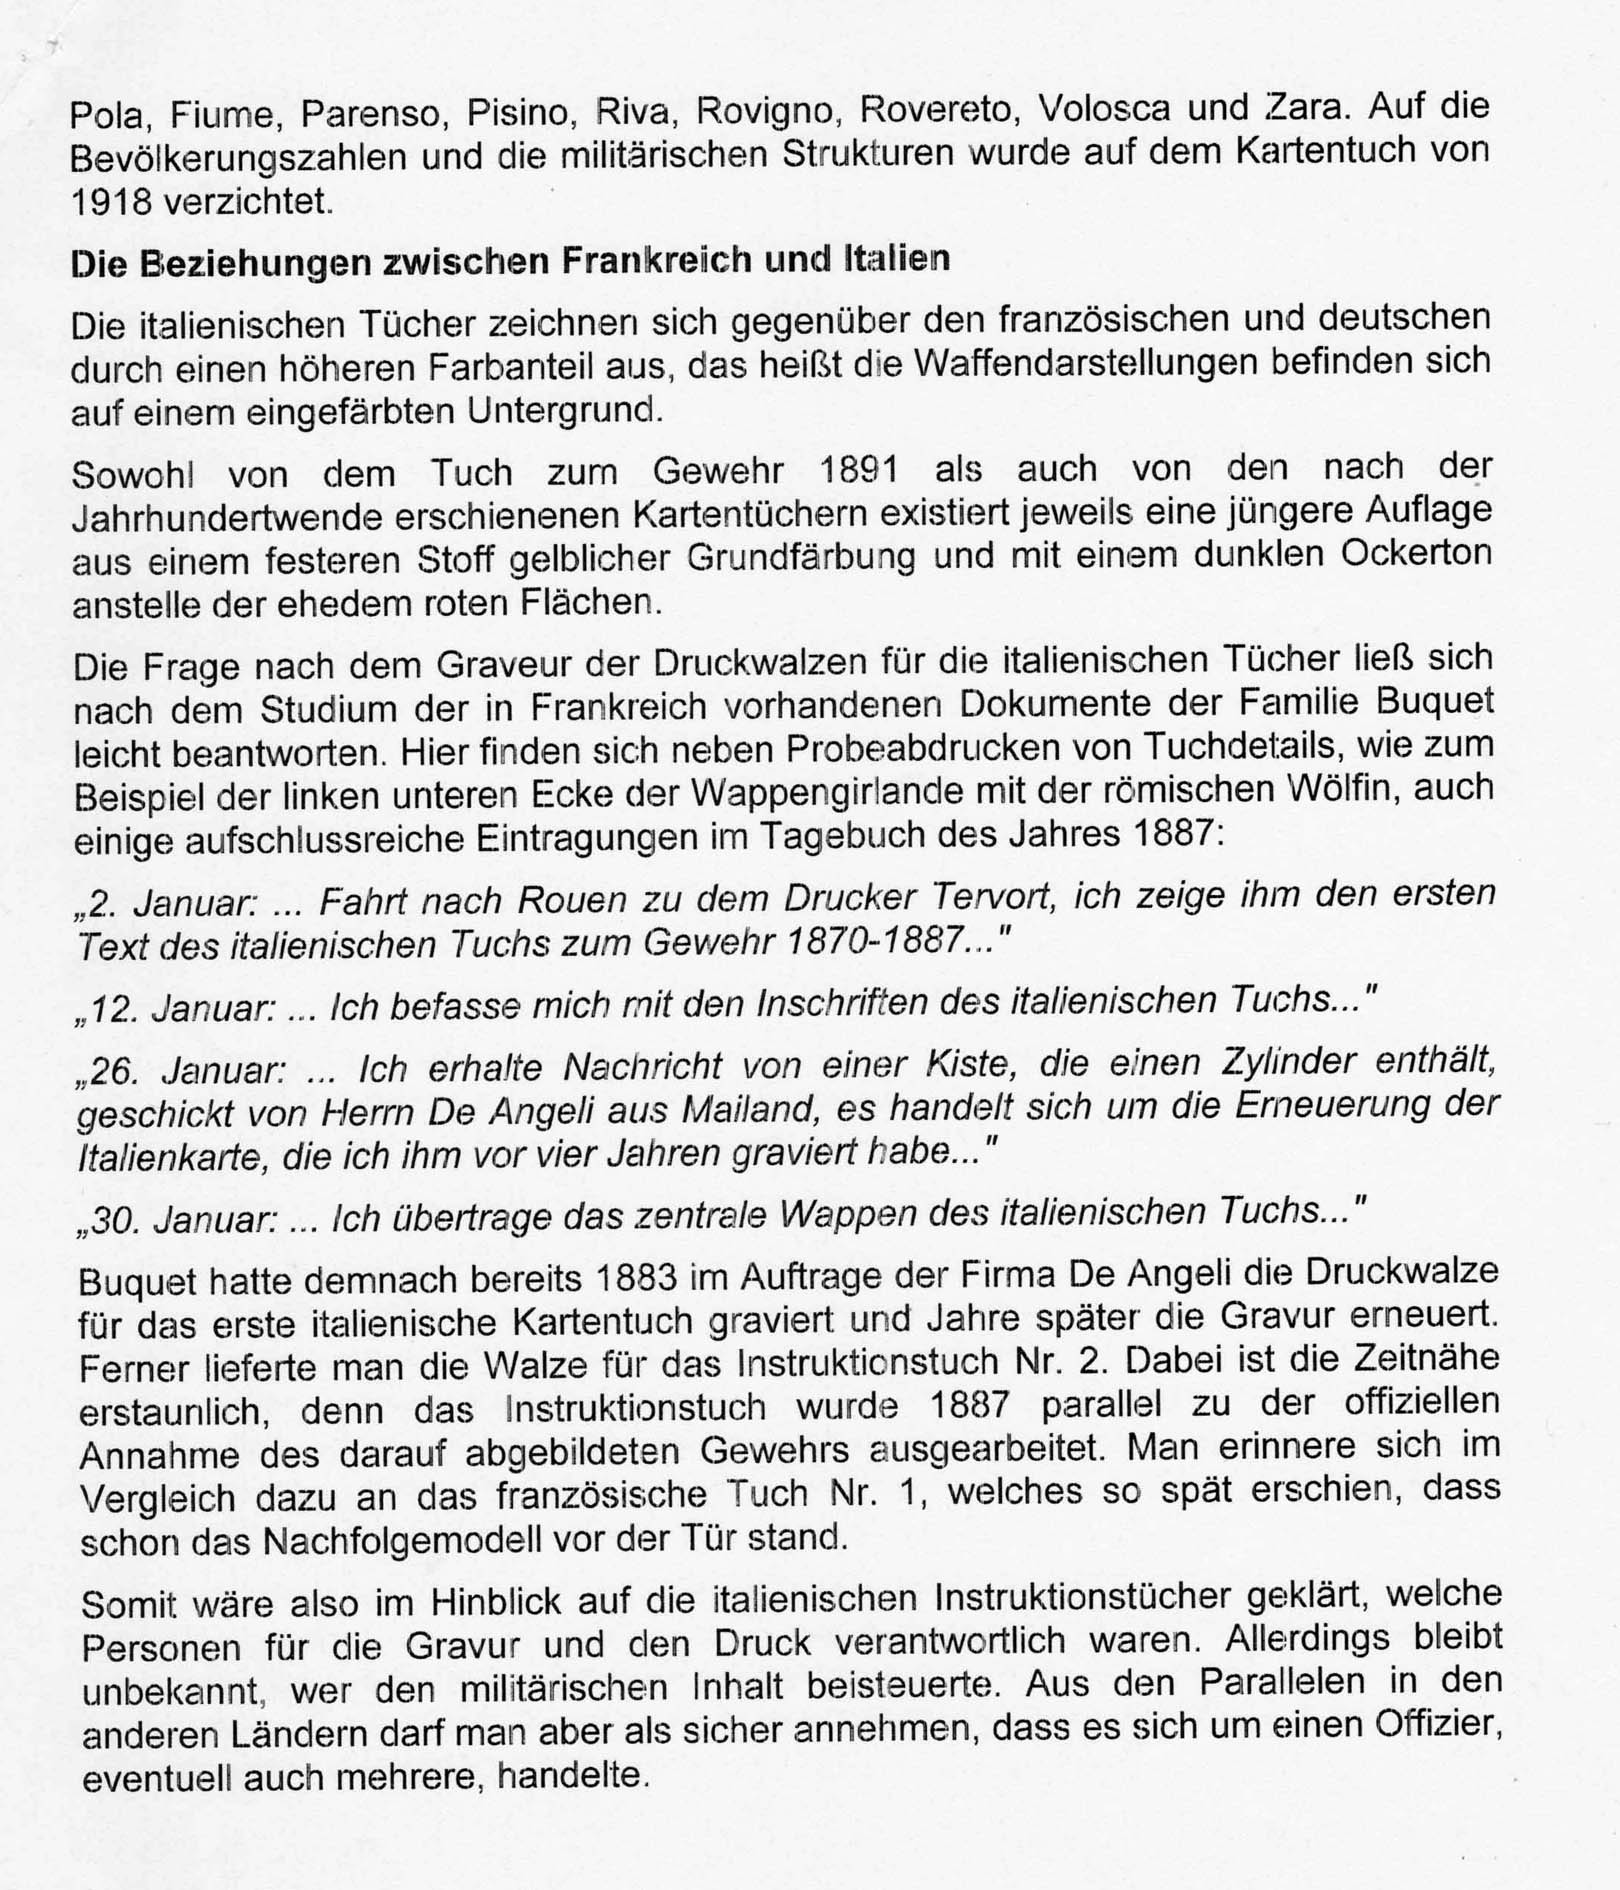
\includegraphics[width=\textwidth]{deangelifrua_8.jpg}
	\caption{}
	\label{fig:deangelifrua_8}
\end{figure}

\newpage

Sul Mediterraneo la Tripolitania deriva dal nome della capitale Tripoli. Questa zona fu annessa nel 1911-1913 sulla scia della guerra italo-turca e della guerra italo-libica. La Tripolitania divenne indipendente col re Idris I nel 1951. Nel 1969 Muammar Gheddafi è arrivato al potere con un colpo di stato militare fondando la Repubblica araba della Libia.

Il fazzoletto italiano con carta geografica del 1918
 (vedi pag.57)

Dopo la fine della prima guerra mondiale in Italia nel 1918, comparve un nuovo fazzoletto, sotto il titolo di "ITALIA - REDENTA ED UNA PER VALORE DEI SUOI SOLDATI - 3 NOVEMBRE 1918". II 3 Novembre 1918 ha segnato con la firma dell'armistizio tra l'Italia e Austria-Ungheria, la fine della prima guerra mondiale su questo fronte.
   Questo fazzoletto porta lungo i bordi il testo "STAMPERIA ITALIANA DE ANGELI MILANO - BREVETTATO".  Questo coincide con un fazzoletto di circa 52 x 52 cm leggermente più piccolo rispetto al suo predecessore. Le colonie non sono più mostrate, ma è stato eseguito un prolungamento a nord con i territori ceduti dall'Austria-Ungheria, l'Alto Adige e l'Istria. Ciò ha aumentato il numero di stemmi in circolo in modo tale che doveva essere aggiunti al fondo di un'altra linea. Ciò comprende i distretti e le nuove città di Ala, Arco, Bolzano, Capodistria, Gorizia, Istria (con errori di stampa), Levico, Pola, Fiume, Parenzo, Pisino, Riva, Rovigno, Rovereto, Volosca e Zara. Sul fazzoletto del 1918 si è rinunciato alla popolazione e alle strutture militari.

I rapporti tra Francia e Italia
  
 I tessuti italiani, in relazione con quelli francesi e tedeschi hanno una maggiore quantità di colore, e ciò significa che gli stemmi sono rappresentazioni su uno sfondo colorato.
   Per il fazzoletto per il fucile nel 1891 così come per quelli pubblicati dopo la fine del secolo, c'è una tiratura più recente di un colore solido di base con un colore giallo ocra scuro al posto dei rosso. La questione dell'incisore dei rulli della stampa per i fazzoletti italiani secondo lo studio dei documenti esistenti fa riferimento alla famiglia francese Buquet. Qui si possono trovare stampe successive di dettagli della stoffa del campione, come ad esempio l'angolo in basso a sinistra dello stemma della lupa romana con la ghirlanda,1 (vedi a pag. 62) e anche alcuni riferimenti nel diario del 1887:  
   “2 Gennaio: ... viaggio a Rouen alla stamperia Tervort, io gli mostro il primo testo del fazzoletto italiano per il fucile 1870-1887... " 
   “12 Gennaio:... Ho a che fare con le iscrizioni del tessuto italiano..”
   “26 Gennaio: ... Ottengo un messaggio di risposta che contiene un cilindro, inviato dal signor De Angeli a Milano, per rinnovare la carta d'Italia, che ho inciso quattro anni fa ...
,, 30 Gennaio:... Trasferisco l'emblema centrale del fazzoletto italiano ...”
   Buquet aveva così inciso nel 1883 per conto di De Angeli, il rullo di pressione per la carta geografica del primo fazzoletto italiano e anni dopo, ha rinnovato l'incisione. Inoltre è stato consegnato il fazzoletto delle istruzioni n ° 2. Qui il poco tempo trascorso è sorprendente, perché nel 1887 è stato preparato il fazzoletto di istruzioni in parallelo con l'adozione formale della carabina raffigurata in esso. Richiama in confronto il fazzoletto francese n ° 1, che sembrava così in ritardo, che c'era già un successore alla porta.
   Così si spiegherebbe in termini di fazzoletti d'istruzione italiani, che le persone che si occupavano di incisione e stampa erano responsabili. Tuttavia, rimane sconosciuto chi abbia contribuito al contenuto militare. Per i paralleli con altri paesi, dobbiamo dare per scontato che si trattasse di un ufficiale, forse anche più d'uno.

\newpage

\begin{figure}[h]
	\centering
		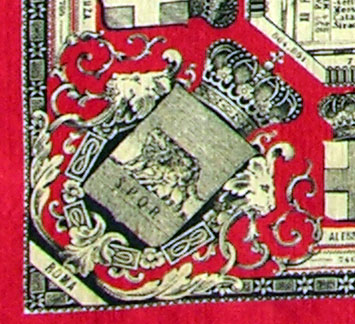
\includegraphics[width=\textwidth]{fazzoletto1_dettaglio.jpg}
	\caption{Dettaglio dell’angolo in basso a sinistra del fazzoletto n°1 (veder pag. 40)}
	\label{fig:fazzoletto1_dettaglio}
\end{figure}

\newpage

\begin{figure}[h]
	\centering
		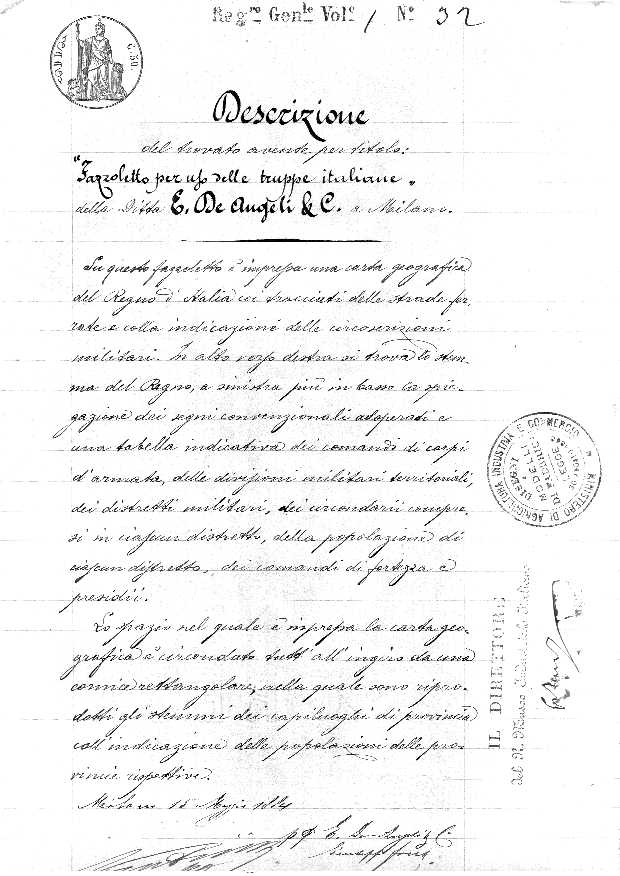
\includegraphics[width=\textwidth]{fazzoletto1_lettera.jpg}
	\caption{15 maggio 1884 Invio al ministero competente della descrizione dettagliata dei contenuti  del fazzoletto n°1}
	\label{fig:fazzoletto1_lettera}
\end{figure}

\newpage

\begin{figure}[h]
	\centering
		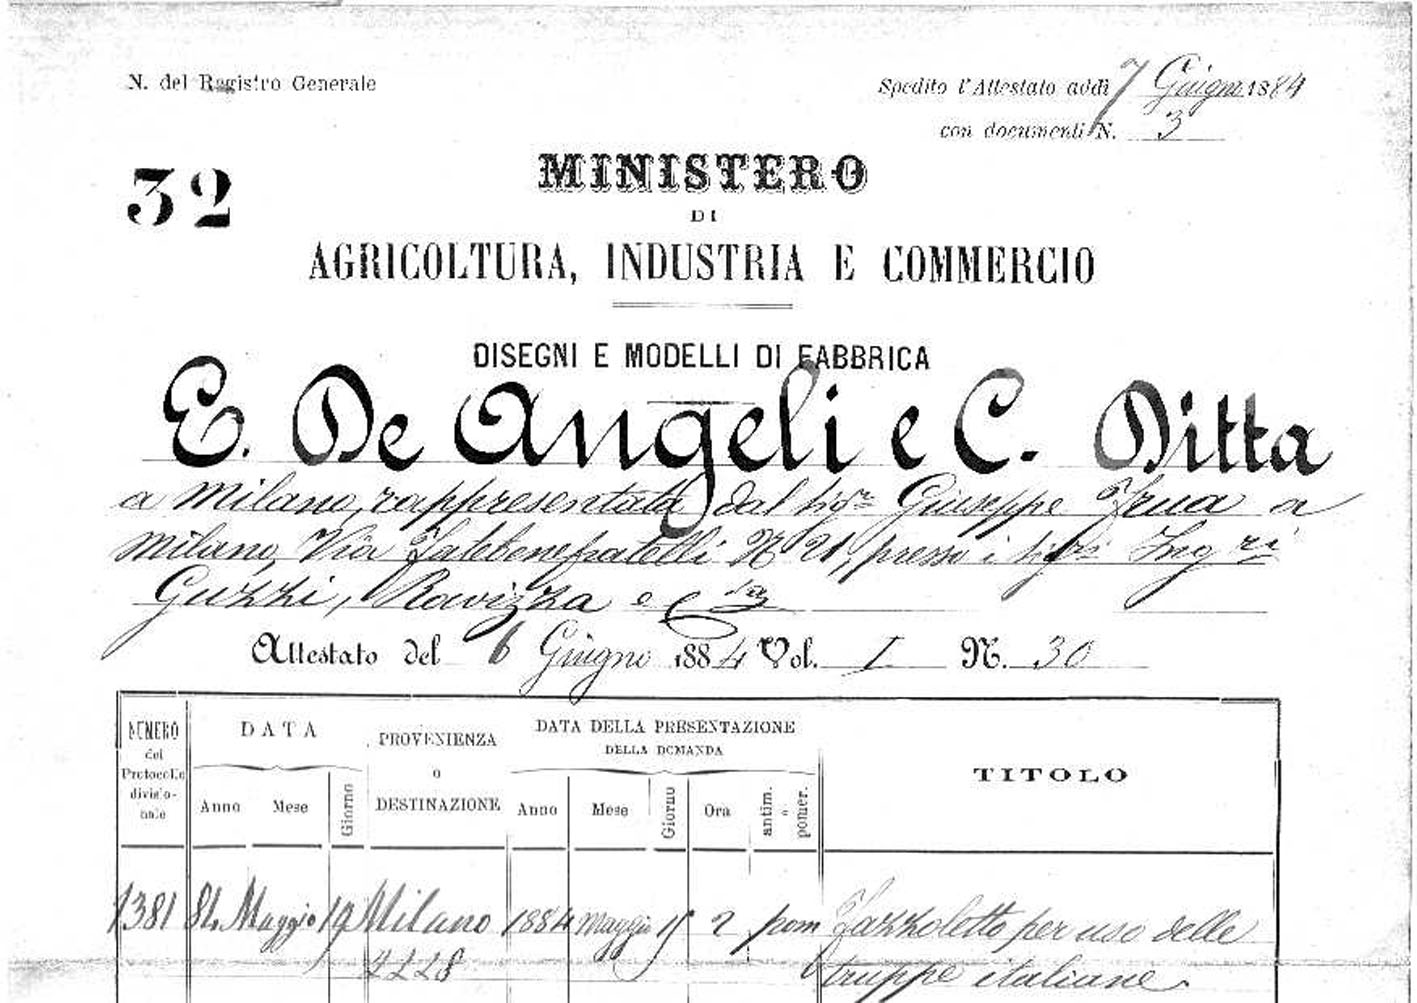
\includegraphics[width=\textwidth]{richiestaautorizzazionestampa.jpg}
	\caption{6 giugno 1884 Richiesta da parte di Giuseppe Frua al ministero competente, per autorizzazione alla stampa dei fazzoletti per istruzione militare italiana}
	\label{fig:richiestaautorizzazionestampa}
\end{figure}

\clearpage







   
   
